% This is samplepaper.tex, a sample chapter demonstrating the
% LLNCS macro package for Springer Computer Science proceedings;
% Version 2.21 of 2022/01/12
%
\documentclass[runningheads]{llncs}
%
\usepackage[T1]{fontenc}
% T1 fonts will be used to generate the final print and online PDFs,
% so please use T1 fonts in your manuscript whenever possible.
% Other font encondings may result in incorrect characters.
%
\usepackage{hyperref}

% Luke added these packages
\usepackage{amssymb}
\usepackage{graphicx}
\usepackage{xcolor}
\graphicspath{ {./figures/} }
\usepackage{subcaption}
\usepackage{amsmath}

\newcommand{\arun}[1]{\textcolor{red}{Arun's note: #1}}
\newcommand{\luke}[1]{\textcolor{blue}{#1}}
\newcommand{\rakib}[1]{\textcolor{teal}{#1}}
\newcommand{\sasha}[1]{\textcolor{olive}{#1}}

\newcommand{\myname}{PUMiNet}

% Used for displaying a sample figure. If possible, figure files should
% be included in EPS format.
%
% If you use the hyperref package, please uncomment the following two lines
% to display URLs in blue roman font according to Springer's eBook style:
%\usepackage{color}
%\renewcommand\UrlFont{\color{blue}\rmfamily}
%\urlstyle{rm}
%
\begin{document}
%
\title{PileUp Mitigation at the HL-LHC\\ Using Attention for Event-Wide Context}
%
%\titlerunning{PileUp Mitigation at the HL-LHC}
% If the paper title is too long for the running head, you can set
% an abbreviated paper title here
%

  \author{Luke Vaughan \textsuperscript{1} \and
  Mohammed Rakib \textsuperscript{2} \and
  Shivang Patel \textsuperscript{1} \and
  Flera Rizatdinova \textsuperscript{1} \and
  Alexander Khanov \textsuperscript{1} \and
  Arunkumar Bagavathi \textsuperscript{2}%\orcidID{0000-0002-7135-4602}
  }

 \authorrunning{L. Vaughan, M. Rakib, S. Patel, F. Rizatdinova, S. Khanov, A. Bagavathi}


  \institute{\textsuperscript{1} Department of Physics, \textsuperscript{2} Department of Computer Science \\
  Oklahoma State University \\
  \email{\{luke.vaughan, mohammed.rakib, shivang.patel, flera.rizatdinova, alexander.khanov, abagava\}@okstate.edu}}


\maketitle              % typeset the header of the contribution
%
\begin{abstract}
%\begin{itemize}
%    \item Abstract should be only 150-200 words
%    \item What Physics problem are we studying? 
%    \item Why is it important? 
%    \item Research gap in the existing works
%    \item What are we innovating in this paper? 
%    \item Our achievements
%    \item Impact on the scientific groups
%    \item Only three keywords
%\end{itemize}
Collider-based experiments play a crucial role in investigating the fundamental properties of the universe. The Large Hadron Collider (LHC) collides bunches of protons that lead to multiple interactions that occur practically simultaneously and overlay on top of the collision of interest for physicists. This creates a pileup effect that makes physics measurements distorted by the products of pileup collisions. In order to improve the discovery potential of the LHC, it is necessary to mitigate the effect of these pileup interactions on the processes of interest. In this paper, we suggest a novel AI-based method, \myname{}, to tackle the problem of the pileup at the current LHC and future High Luminosity LHC conditions. \myname{} is an attention-based algorithm that mitigates pileup effects using a regression task on jets in the context of an entire event.

\keywords{Pileup Mitigation  \and Attention NN \and HL-LHC.}
\end{abstract}
%
%
%
\section{Introduction}\hfill

% The Large Hadron Collider~\cite{LHC}, LHC, is the largest and highest energy particle collider ever constructed by humankind. Using superconducting magnets, protons are accelerated around a 27km ring and collide in designated interaction points at a center of mass energy of 14TeV. The proton-proton interactions produce heavy particles which decay into a higher multiplicity of lighter particles. This decay chain results in a cascading effect which creates a shower of particles observed by the detector. If particles originate from a common heavy ancestor, they often form collimated streams of lighter particles in a tight cone, which are referred to as jets.

At the Large Hadron Collider, LHC, the ATLAS and CMS experiments look at the interactions of elementary particles to better understand the fundamental structure of nature. These studies are performed by colliding groups of protons, or bunches, at extremely high energies. At such high energy, each collision leads to the production of hundreds of particles which are registered by the ATLAS and CMS detectors. The information recorded by the detectors are referred to as an \emph{event}. Since each bunch contains $10^{11}$ protons, each event contains information from multiple proton-proton interactions. The average number of interactions per bunch crossing recorded in an event is referred to as $\left\langle \mu \right\rangle$. The events selected for recording are chosen in such a way that at least one of these interactions is a \emph{hard scatter}, considered as \emph{signal}, which contains highly energetic particles that are of interest to physics. Other interactions recorded in the same event are called \emph{pileup}, considered as \emph{background}, which contaminates the signal.

\begin{figure}[ht]
\centering
  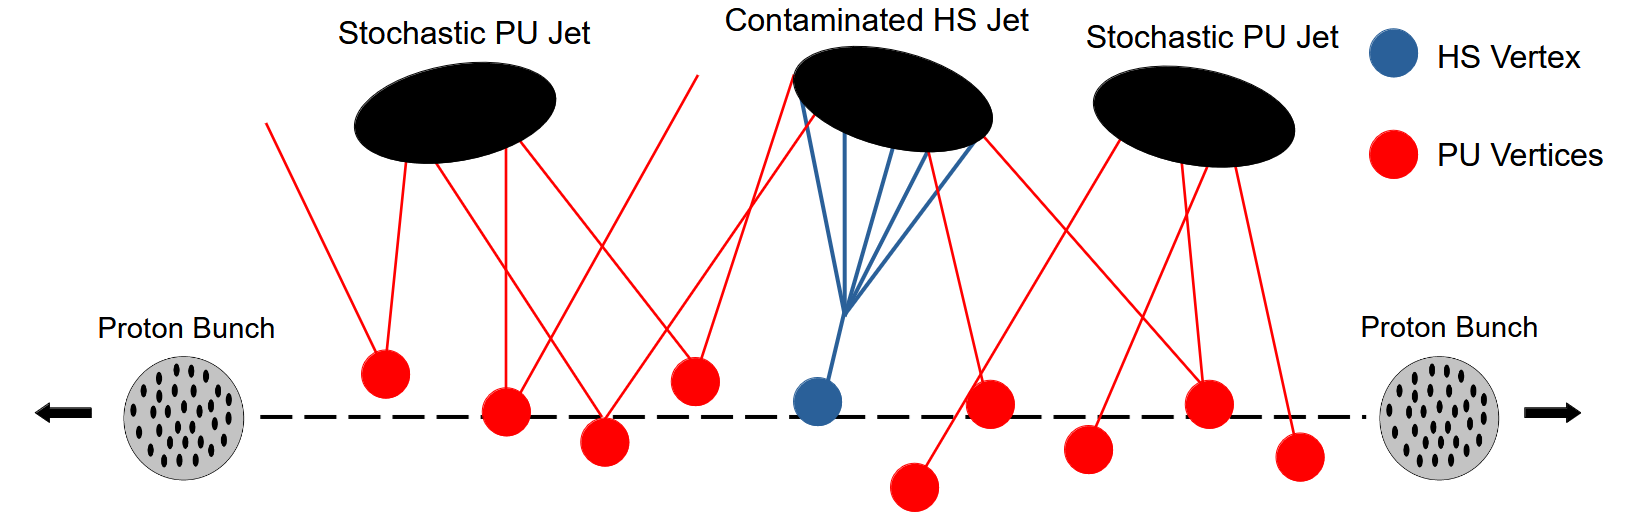
\includegraphics[width=1\linewidth]{Pileup_Graphic.png} 
  \caption{The interactions from crossing proton bunches in a single event. Hard scatter, HS, interaction originates from the primary vertex while other interactions, PU, originate from pileup vertices. The jets that originate from the HS vertex form a correlated set, while the jets from PU are stochastic in nature and do not have correlations.}
\label{fig:PileupJets}
\end{figure}

Our research focuses on physics processes where particles form streams that can be clustered into tightly knit cones called \emph{jets}, which can originate from both hard scatter and pileup collisions. Throughout this article, we refer to particles as \emph{tracks}, and the collision points from which the tracks originate as \emph{vertices}. In a real experiment, jets are measured and identified using information from many subdetector systems, but to simplify the problem, in this paper we treat jets purely as sets of tracks. While jets containing tracks due to hard scatter are of actual physics interest, there are many jets originating from the pileup interactions (Figure~\ref{fig:PileupJets}). Pileup mitigation techniques employed so far typically follow a two-step approach: (i) a binary classification task to identify jets as hard scatter or pileup~\cite{ATLAS-CONF-2014-018}, and (ii) application of energy and mass corrections to jets identified as hard scatter through algorithms such as Charged Hadron Subtraction~\cite{CHS}.

%\arun{Should we remove this last sentence as we detail about this in the next paragraph? Instead, shall we give a sentence motivation for jet level binary classification problem?} The main purpose of this study is (1) to identify the jets from hard scatter and pileup and (2) to measure the level of contamination of hard scatter jets from pileup tracks.

%At the Large Hadron Collider (LHC)~\cite{LHC}, physicists study to better understand phenomena of the universe related to the fundamental forces of nature. These proton-proton collisions produce elementary particles that are irreducible quanta of energy.
%described by the Standard Model of Particle Physics. 
%Due to the subatomic size of protons, the mean number of interactions per bunch crossing, $\left\langle \mu \right\rangle$, is very small. Only one of these collisions interacts via a strong head-on collision that produces deep inelastic scattering called \emph{hard scatter} or \emph{signal}, while other weaker interactions are called \emph{pileup} or \emph{background}. 
%In addition to hard scatter, there exists many other soft collisions arising from weaker interactions which are called \emph{pileup}. 

%Each of these collisions, in turn, produces heavy particles which decay into lighter particles in a cascading effect. Streams of such decayed particles are called \emph{jets}, which can be clustered to form a tightly knit cone containing charged particles, called \emph{tracks}. All these collisions are recorded as \emph{events}, usually at a rate of every 25 nanoseconds, containing a variable number of jets and a variable number of tracks in each jet. It is important to note that jets originating from hard scatter processes share underlying physics and thus can be correlated with other jets in the hard scatter process. Such a correlation is not feasible for pileup jets due to their stochastic nature, as given in Figure~\ref{fig:PileupJets}.

%The Large Hadron Collider~\cite{LHC}, LHC, is the largest and highest energy particle collider ever constructed by humankind. Using superconducting magnets, protons are accelerated around a 27km ring and collide in designated interaction points at a center of mass energy of 14TeV. This decay chain results in a cascading effect which creates a shower of particles observed by the detector.
%The proton-proton interactions that happen in colliders like Large Hadron Collider~\cite{LHC} produce heavy particles which decay into a higher multiplicity of lighter particles in a cascading effect. 
%\textcolor{red}{We need to simplify these two sentences.} Streams of such lighter particles originating from a common ancestor are called \emph{jets}, they often form collimated streams of lighter particles in a tight cone, which are referred to as jets.

%General purpose detectors at the LHC consist of two main components: a tracker and a calorimeter. The tracker uses silicon dots and strips to measure the position and momentum of each particle that passes through it. Particles that are reconstructed using the tracker are referred to as tracks. The calorimeter uses dense material, such as lead, to absorb and record the energy of particles. A stream of collimated particles that deposits energy into the calorimeter is reconstructed as a jet.

%Due to the very small interaction cross-section of proton-proton collisions, bunches of 100 billion protons are collided at the same time to increase the rate of interaction. On average, there will be zero or one collisions that interact "head on" producing deep inelastic scattering. This type of interaction is called the Hard Scatter, HS, process. However, in the current LHC configuration, there exists, on average, an additional 60 other interactions from various protons in the bunch crossing that are physically piled up on top of the hard scatter interaction. These additional interactions are referred to as Pileup, PU, processes.



%Pileup interactions are considered as contamination because of their ample quantities compared to signal processes. It is important to identify and mitigate pileup from each collision events to increase sensitivity of signal processes and assist physicists to discover new particles. 

%Machine learning and AI methods have been introduced in recent years to help physicists analyze data at the LHC. Machine learning has been applied to several sub-problems in High Energy Physics~\cite{he2023high,Larkoski_2020}, such as jet flavor tagging~\cite{ParticleNet}, top tagging~\cite{Barman_2024}, generative event modeling~\cite{kansal2021particle}, and anomaly detection. While machine learning techniques have been applied to analyze pileup~\cite{komiske2017pileup,ABCNet}, methods to analyze \emph{PileUp} at large $\left\langle \mu \right\rangle$ values have been mostly overlooked in the existing works. Although there is growing interest in this domain due to upcoming LHC upgrades, existing methods assume (i) only low pileup events, and (ii) pileup identification as a binary classification problem. As LHC prepares to upgrade to the High-Luminosity (HL)LHC~\cite{HLLHC}, with $\left\langle \mu \right\rangle = 200$, it brings exponentially higher number of pileup particles per event.

The LHC prepares to upgrade to the High-Luminosity phase, HL-LHC, where $\left\langle \mu \right\rangle$ will increase from 60 to 200. This upgrade will dramatically increase the number of pileup particles in each event, which will increase the statistics of rare hard scatter processes. However, in order to maximize the discovery potential of the HL-LHC, there is a need to mitigate high pileup conditions: in particular, to quantify the energy and momentum contributions from pileup to hard scatter jets. Existing methods have focused on investigating pileup at $\left<\mu\right>$ values below 60 ~\cite{ATLAS-CONF-2014-018}, but as $\left<\mu\right>$ approaches 200, the high pileup conditions degrade the quality of hard scatter jets to the point that binary classification is no longer suitable. The large pileup background shifts the problem to a continuous regression task which, in  turn, performs the simultaneous tasks of identification, energy correction, and mass correction of hard scatter jets.

Machine learning methods have become widespread in High Energy Physics, HEP, ~\cite{he2023high,Larkoski_2020} assisting with pileup mitigation~\cite{komiske2017pileup}, jet tagging~\cite{ParticleNet}, top tagging~\cite{Barman_2024}, event modeling~\cite{kansal2021particle} and searches for new physics using anomaly detection~\cite{duarte2024novelmachinelearningapplications} and other AI methods. The ATLAS experiment is using the JVT kNN algorithm~\cite{ATLAS-CONF-2014-018} which relies on constructing high level variables using track and jet features to perform binary classification on a per jet basis.  However, this method fails to incorporate correlations between jets and tracks at the event level. There have been attempts to introduce correlations between tracks and jets using graph neural networks~\cite{ParticleNet,ABCNet}, however, it has been shown~\cite{qu2022particle} that attention neural networks scale more efficiently which is a requirement for high pileup conditions.

This work proposes an attention-based neural network, \myname{}, to mitigate pileup by performing the simultaneous identification, energy correction, and mass correction of hard scatter jets. \myname{} uses self and cross attention to capture all possible correlations between jets and tracks within an entire event while maintaining good performance when scaling to high pileup conditions. \myname{} also outperforms benchmarks against existing methods in our experiments, and increases the discovery potential of the HL-LHC through a practical example of a physics analysis.

%\textcolor{violet}{In this work, we present the following contributions:
%\begin{enumerate}
%    \item We propose a first-of-its-kind pileup prediction modeled as a regression problem.
%    \item We propose cross-attention based neural network architecture that utilizes jets and tracks information for pileup fraction detection.
%    \item We show with extensive analysis that the proposed method outperforms the baseline approaches.
%    \item We also show that the predictions from the proposed approach also assist with physics processes.
%\end{enumerate}}


%\arun{I think there was a few sentences approximately how many millions/billions of collisions per proton bunch. That was interesting and would look good if we have it in one sentence in next paragraph.}

 
 %\luke{In low pileup conditions, the data is sparse such that jets can be easily binary classified as hard scatter or pileup jets. There could be a few pileup tracks entering a hard scatter jet, which can be corrected using Charged Hadron Subtraction~\cite{CHS}, but the overall mass and energy of the hard scatter jet are seemingly unaffected. This becomes challenging with the upcoming upgrades to LHC which introduces several noisy pileup tracks into hard scatter jets and eventually altering core properties of hard scatter jets.}


%\luke{In low pileup conditions, pileup is sparse enough such that jets tend to be binary classified as hard scatter or pileup jets as shown in figure \ref{fig:PileupJets}. There could exist a few tracks entering a hard scatter jet, which can be corrected using Charged Hadron Subtraction~\cite{CHS}, but the overall mass and energy of the hard scatter jet are seemingly unaffected. However if pileup increases, there exists a critical point in $\left\langle \mu \right\rangle$ where there is such a large pileup background that the mass and energy of hard scatter jets are significantly affected.}
%This critical point becomes more daunting as the LHC prepares to upgrade to the High-Luminosity (HL)LHC~\cite{HLLHC}. The HL-LHC will bring in much more data for hard scatter collisions at the cost of many more pileup collisions.

%\luke{The existing algorithms developed for pileup mitigation using binary classification at low pileup conditions for the LHC will start to struggle as pileup is increased for the HL-LHC. Therefore at high pileup conditions, future algorithms must consider pileup as continuous regression problem to determine by what fraction the \emp{hard scatter} jet's mass and energy has been affected by \emp{pileup}. In this paper we propose a model that attempts to solve the problem of pileup by directly predicting energy and mass fractions of each jet using transformer encoders using self-attention and cross-attention to learn enriched representations of jets using all possible correlations between jets and tracks within the context of an event.}

% \arun{Explain why it is necessary to identify pileup jets for physics processes.} \luke{Processes that lead to new physics, considered as signal, occur through \emph{hard scatter} interactions. All other interactions are considered \emp{pileup} and are a source of background which contaminates the signal. Therefore, the identification and suppression of the \emp{pileup} background is crucial to increase the sensitivity to signal of the \emp{hard scatter} processes. Pileup mitigation helps physicists to probe new physics and discover new particles by reducing the pileup background.}

%An event is defined as data recorded from a single bunch crossing which occur every 25 nanoseconds. Each event contains variable length set of jets. Each jet contains a variable length set of tracks. The hard scatter jets that originate from the same underlying physics process will be correlated with each other. On the other hand, pileup jets are formed due to stochastic nature and are not correlated to other jets in the event. Attention neural networks are capable of learning correlations between jets and allow for a context window of an entire event.

% \begin{figure}[h]
%   \centering
%   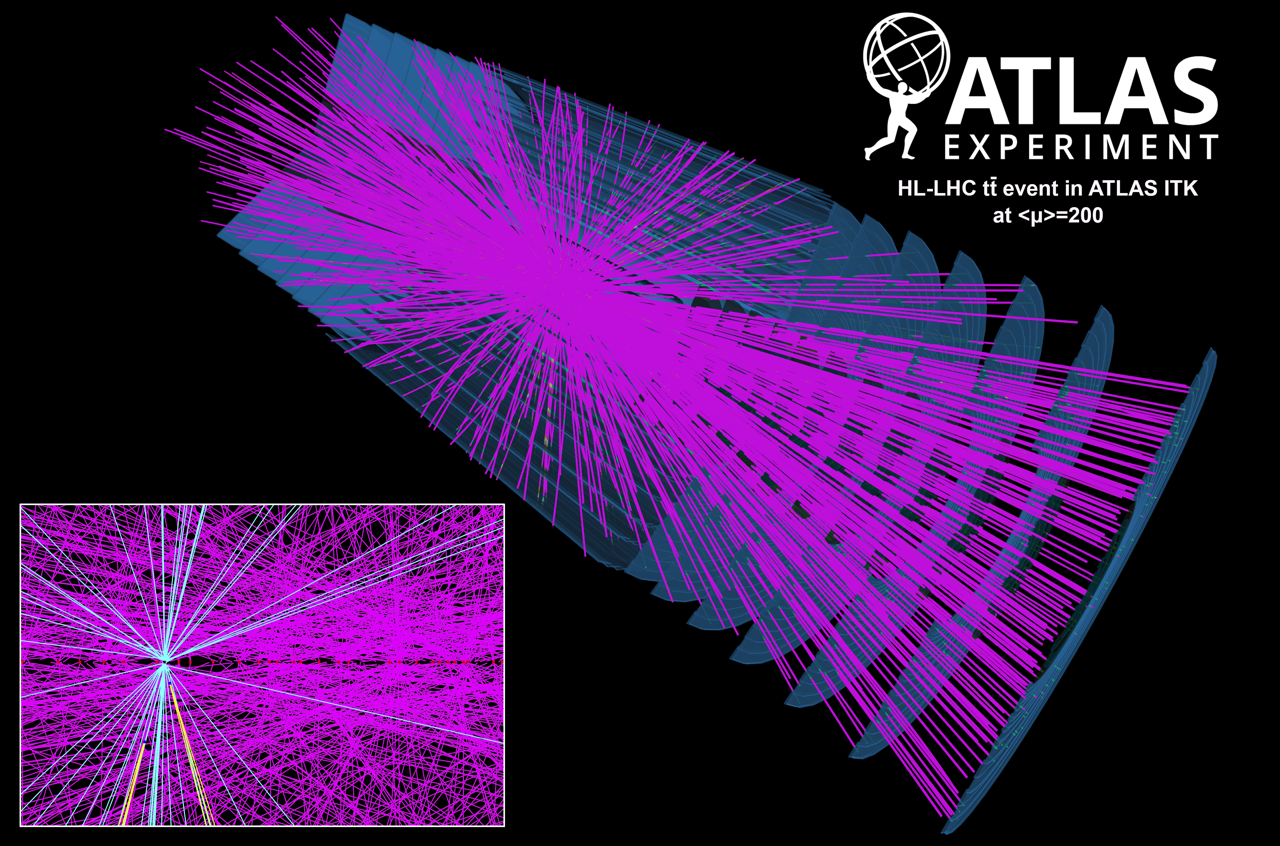
\includegraphics[width=0.75\linewidth]{HL-LHC-tt}
%   \label{fig:vertexing}
%   \caption{In the HL-LHC configuration, the Hard Scatter process (light blue) begins to be dominated by PileUp (purple). Note: https://atlas.cern/updates/news/scientific-potential-high-luminosity-lhc}
% \end{figure}

%In order to increase the amount of data collected, the LHC has plans to plans to increase the mean number of collisions, $\left<\mu\right>$, for what is called the High-Luminosity (HL)LHC~\cite{HLLHC}. The HL-LHC will increase the mean number of interactions up to $\left<\mu\right>=200$ to collect more data and increase statistics. This change in configuration of the LHC will bring much more pileup begins to dramatically blur the concept of a HS and PU jet. What was a binary classification task at low pileup conditions becomes a continuous regression task at high pileup conditions. This is due to the fact that there are so many pileup particles crammed into the $4\pi$ solid angle coverage of the detector, that nearly all hard scatter jets have a significant contribution to their mass and energy from pileup. 

%This motivates that jets should not be considered as binary HS or PU, but instead jets should have a continuous energy and mass corrections that are be applied to correct for pileup effects. In this paper, we propose an improvement to pileup mitigation at the HL-LHC using Multi-Head Attention and Transformer Encoder stacks~\cite{Attention} to perform a continuous regression task on jets in the context of an entire event. \\


%\section{Related Work}\hfill

Machine learning approaches for High Energy Physics problems are gaining traction from multiple perspectives with advancements in neural networks~\cite{he2023high,Barman_2024,Larkoski_2020}. Although there are several sub-problems in High Energy Physics, such as jet flavor tagging~\cite{qu2022particle`}, top tagging, generative event modeling~\cite{kansal2021particle}, unfolding, anomaly detection, and calibration that have been explored with machine learning, methods to analyze \emph{PileUp} have been mostly overlooked in the existing work. One of such interesting problems is mitigating pile-up particles and correcting jet mass and energy for events that occur at the Large-Hadron Collider~\cite{komiske2017pileup}. \\ 

Existing pileup mitigation techniques for the ATLAS and CMS experiments have focused on solving the binary classification problem for either jets or tracks. ATLAS uses algorithms to classify jets using classifiers such as kNN algorithms~\cite{ATLAS-CONF-2014-018} which rely on constructing high level variables on a per jet basis. CMS uses an algorithm to classify tracks using a statistical $\chi^2$ approach through the PUPPI~\cite{Bertolini_2014} algorithm classifies pileup at the particle level. However, these methods fail to incorporate correlations between jets at the Event level for Event-Wide context. Correlations exists between jet originating from Hard Scatter processes.  \\

Graph Neural Networks have also been studied for for pileup mitigation, however, it is non-trivial how to form a graph in the context of an event. Its unfeasible to connect all particles in an event due to computation limitations, and connecting all tracks within a jet can confuse the model unless edge weights are assigned properly for HS and PU particles. Dynamic edge convolutions have been studied, but this can lead to long training times due to calculating kNN in latent space. Attention, on the other hand, gives a highly parallelizable algorithm to automatically determine weights between objects and update node representations accordingly.

\section{Jet Corrections in High Pileup Conditions}\hfill

As $\left<\mu\right>$ increases from 60 to 200 for the HL-LHC upgrade, the pileup contamination of hard scatter jets will begin to dominate. As PU contamination degrades the quality of HS jets, the task shifts from a binary classification at low pileup conditions to a continuous regression at high pileup conditions. Instead of the traditional binary labels as HS or PU, we introduce a continuous labels for Energy and Mass Fraction, Efrac and Mfrac, which represents the fraction of the jets energy and mass originating from pileup.

To construct these continuous labels, we sum over the Lorentz Four-Vector of the tracks, $\vec{T_i} = (E,p_x,p_y,p_z)_i = (E,\vec{p})_i = (T_0, T_1, T_2, T_3)_i$, which are truth-associated to each jet, $\vec{J}$:

\begin{equation}
    \vec{J}_{HS} = \sum_{i \in \text{HS}} \vec{T}_i \phantom{............} \vec{J}_{PU} = \sum_{i \in \text{PU}} \vec{T}_i \\
    %\vec{J}_{Total} = \vec{J}_{HS} + \vec{J}_{PU} 
\end{equation}

Now that we have the four vector HS and PU contributions of each jet, we can directly evaluate the Energy and Mass fractions on a per jet basis. The total Lorentz Four-Vector is simply the sum of the HS and PU contributions, $\vec{J}_{Total} = \vec{J}_{HS} + \vec{J}_{PU}$. Note that Energy is the first component of the jets Four-Vector, $J_0=E$, and mass is found using the relativistic energy relations in natural units, $m^2=E^2-|\vec{p}|^2$. These expressions can be used to derive the labels used for regression.

\begin{equation}   
    Efrac = \frac{E_{HS}}{E_{Total}} \phantom{............} Mfrac = \frac{m_{HS}}{m_{Total}}
\end{equation}

\begin{figure}[h]
\centering
\begin{subfigure}{.35\textwidth}
  \centering
  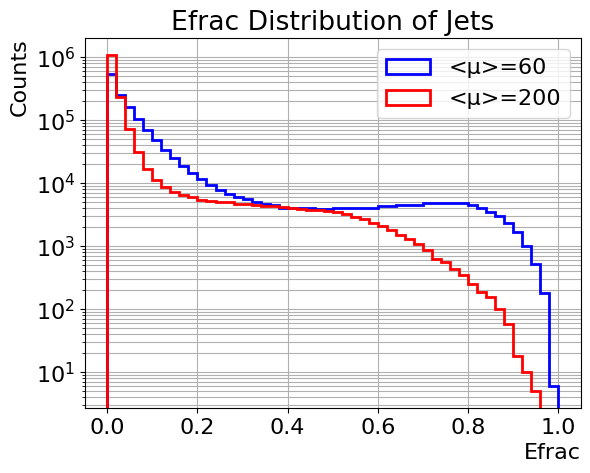
\includegraphics[width=1\linewidth]{Efrac}
  \caption{}
  \label{fig:sub1}
\end{subfigure}%
\begin{subfigure}{.35\textwidth}
  \centering
  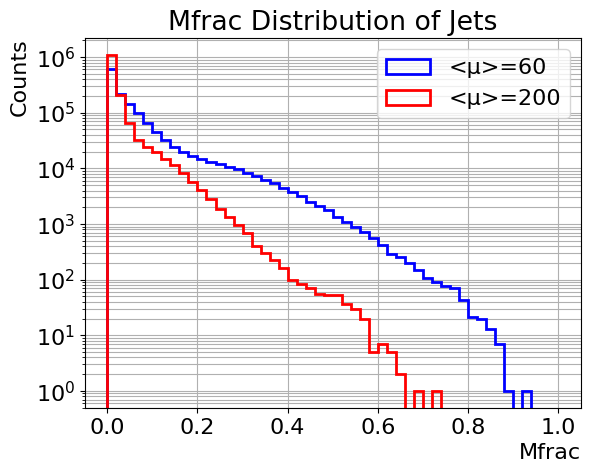
\includegraphics[width=1\linewidth]{Mfrac}
  \caption{}
  \label{fig:sub2}
\end{subfigure}
\caption{The truth energy and mass fractions used for the continuous regression task at $\left< \mu \right> = 60$.}
\label{fig:test}
\end{figure}

These continuous labels allow for corrections to be applied directly to the jet mass and energy. Of course a proper calibration will need to be applied when evaluated on data.


\section{Simulated Dataset}\hfill

A sample of 100k $pp \rightarrow HH$ events were generated using MADGRAPH\_AMC@NLO~\cite{Alwall_2014} and showered through $H \rightarrow b\bar{b}$ channel using Pythia8~\cite{bierlich2022comprehensiveguidephysicsusage}. As each hard scatter process is showered in Pythia, pileup processes are overlaid using SoftQCD:inelastic generated with the A14 central tune with NNPDF2.3LO~\cite{bierlich2022comprehensiveguidephysicsusage}. The average number of pileup processes are controlled by parameter $\left<\mu\right>$ which follows a poisson distribution. Each pileup vertex undergoes gaussian smearing where the width in the x and y directions, representing the beam width, are 0.3mm and the spread in the z direction is 50mm. Stable final state particles are then passed to FastJet~\cite{Cacciari_2012} to be cluster into jets using $anti-k_t$ algorithm~\cite{Cacciari_2008} with R=0.4 and minimum $p_T$ of 25 GeV. \\

\begin{figure}[h]
\centering
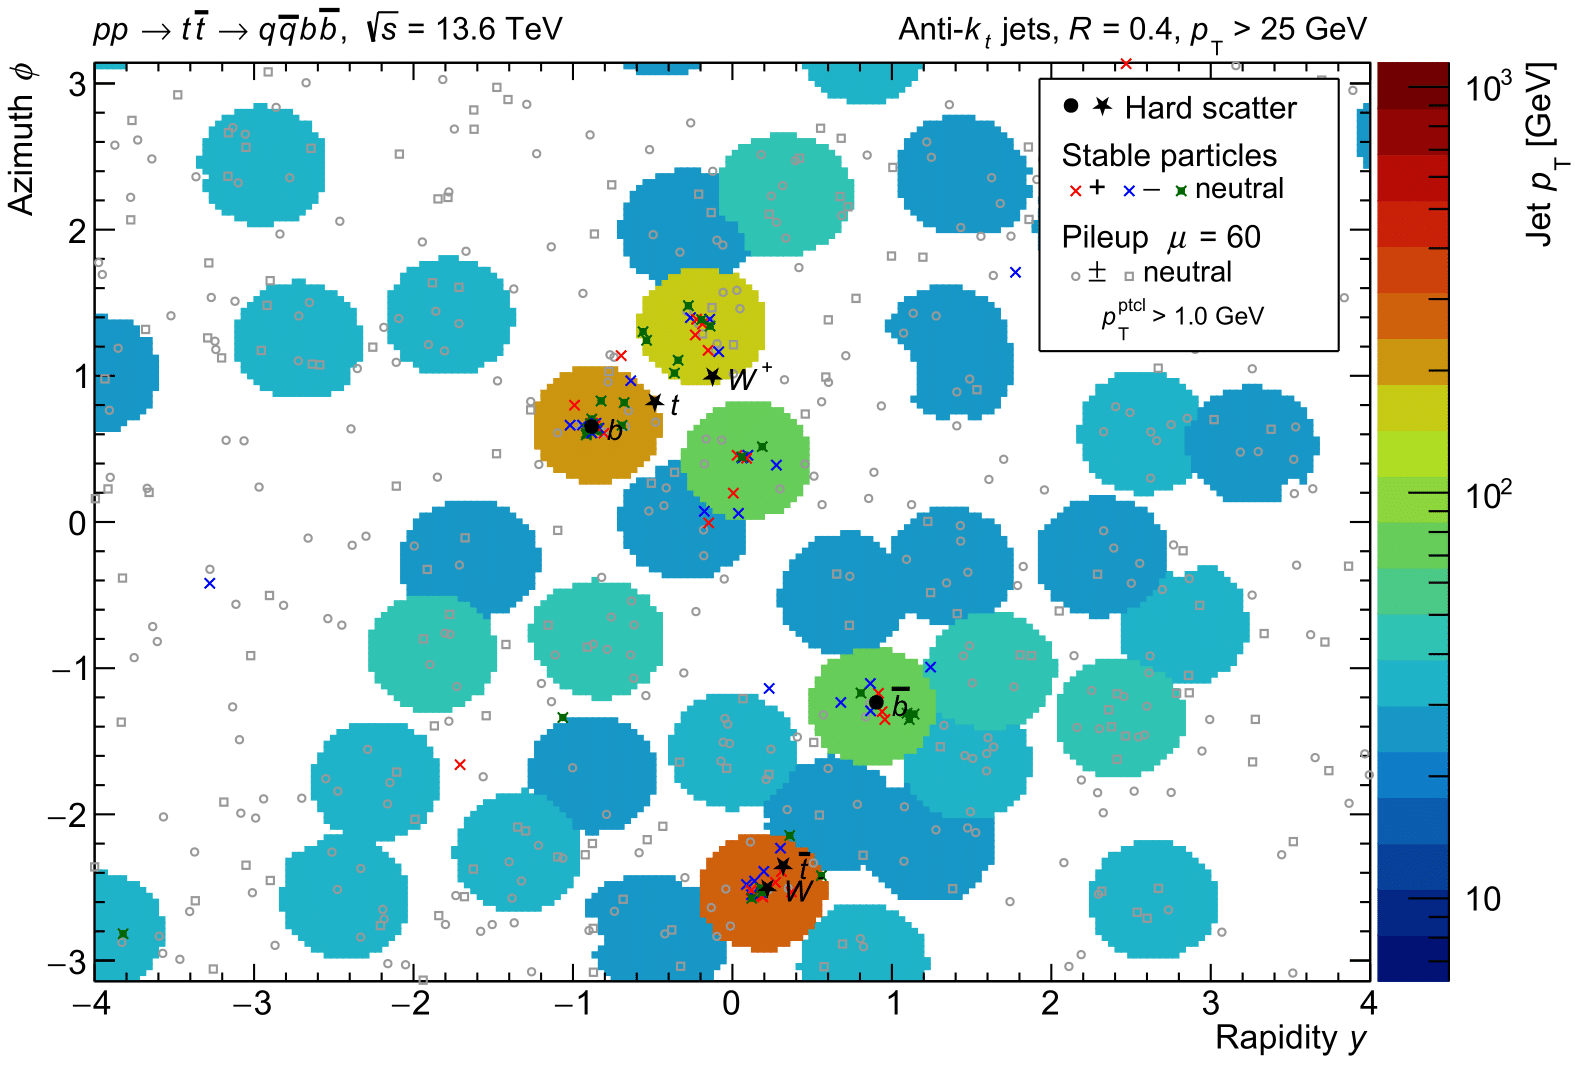
\includegraphics[width=0.65\textwidth]{Event}
\caption{An example of a simulated event of $pp \rightarrow t\bar{t}$ decaying hadronically at $\left< \mu \right> =60$.}
\end{figure}

To incorporate detector limitations, neutral particles and particles below 400 MeV were cut from the training dataset. After cuts, the dataset contains 500k jets and 10M particles. However, it is important to note that the jets studied in this paper are not calorimeter jets, but instead more idealistic track-jets. The results from this study offer the best-case scenario when tracks can be perfectly assigned the correct vertex, and the performance would be expected to degrade slightly in realistic detector conditions.

%\section{Improving JVT using Attention}\hfill

The JVT model used by ATLAS is used to classify jets as HS or PU. However, in high pileup conditions JVT algorithm will need to be improved. Here we benchmark the JVT kNN algorithm~\cite{ATLAS-CONF-2014-018} against AttnJVT.

%\subsection{Jet Features}\hfill
%Each jet has 6 features which includes the kinematic 4-vector of each jet, $p_T, \eta, \phi, m$ as well as track dependent features $corrJVF, Rp_T$ which were first proposed by ATLAS~\cite{ATLAS-CONF-2014-018}. First, corrJVF can be understood as the fraction of the jet's momentum coming from hard scatter particles originating from the primary vertex with respect to the total momentum coming from all other vertices. However, it has been shown that this variable has a dependence on $\left<\mu\right>$, so to correct for this behavior the contribution from pileup vertices are normalized by the number of pileup particles in the event and a free parameter, k. This parameter has been shown to best remove dependence on $\left<\mu\right>$ at k=0.01~\cite{ATLAS-CONF-2014-018}.
%\begin{equation}
%    corrJVF = \frac{\sum\limits_k p_T^{trk_k}(PV_0)}{\sum\limits_l p_T^{trk_l}(PV_0)+\frac{\sum\limits_{n\geq1}\sum\limits_l p_T^{trk_l}(PV_n)}{(k \cdot n^{PU}_{trk})}}
%\end{equation}

%\begin{figure}[h!]
%\centering
%\begin{subfigure}{.45\textwidth}
%  \centering
%  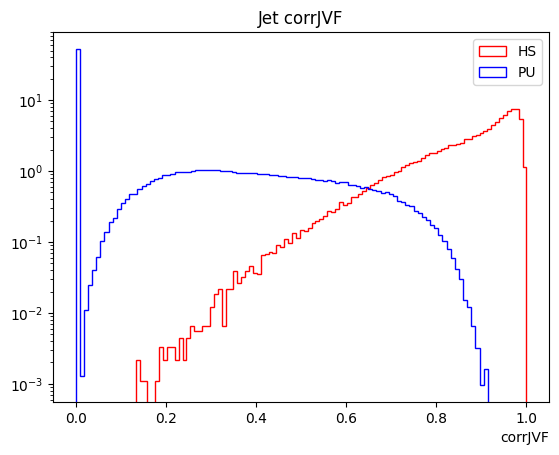
\includegraphics[width=0.9\linewidth]{corrJVF}
%  \caption{}
%  \label{fig:sub1}
%\end{subfigure}
%\begin{subfigure}{.45\textwidth}
%  \centering
%  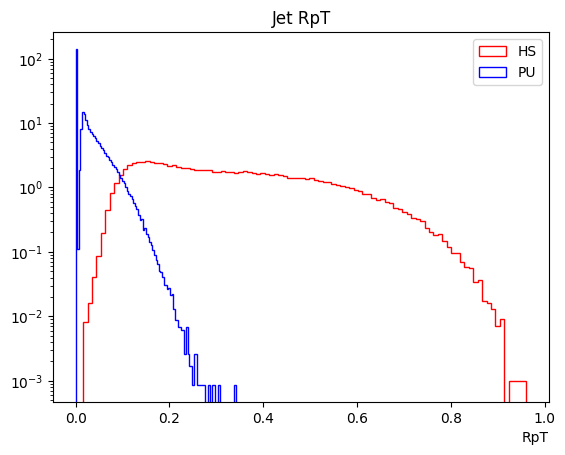
\includegraphics[width=0.9\linewidth]{RpT}
%  \caption{}
% \label{fig:sub2}
%end{subfigure}
%\caption{Figure (a) The distribution of corrJVF for Hard Scatter jets and PileUp jets.. Figure (b) The %istribution of $R_{pT}$ for Hard Scatter jets and PileUp jets.}
%label{fig:test}
%\end{figure}

%Second, $R_{pT}$ can be understood as the fraction of the jet's momentum originating from hard scatter primary vertex.
%\begin{equation}
%    R_{pT} = \frac{\sum_kp_T^{trk_k}(PV_0)}{p_T^{jet}}
%\end{equation}

%These features have unique distributions for HS and PU jets. HS jets tend to have higher corrJVF and RpT than pileup jets as shown in figure [*]. \\

%\begin{figure}[h!]
%\centering
%\begin{subfigure}{.25\textwidth}
%  \centering
%  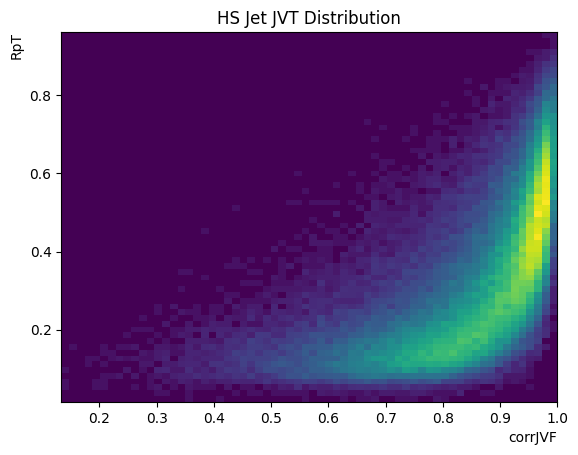
\includegraphics[width=0.9\linewidth]{HS}
%  \caption{}
%  \label{fig:sub1}
%\end{subfigure}%
%\begin{subfigure}{.25\textwidth}
%  \centering
%  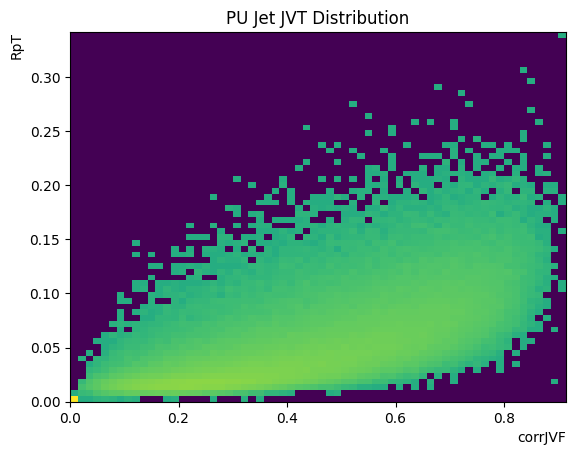
\includegraphics[width=0.9\linewidth]{PU}
%  \caption{}
%  \label{fig:sub2}
%\end{subfigure}
%\caption{Distribution of jets in the $R_{pT}$-corrJVF plane for (a) HS and (b) PU jets.}
%\label{fig:test}
%\end{figure}

\subsection{Jet Labels}\hfill

To fairly benchmark JVT and AttnJVT, a binary label was constructed by cutting on the squared sum of the constituent particle's $p_T$.

\begin{equation}
    PU_{fr} = \frac{\sum\limits_{PU} p_T^{2}}{\sum\limits_{HS} p_T^{2} + \sum\limits_{PU} p_T^{2}}
\end{equation}

An arbitrary cut is imposed on this distribution to convert the continuous distribution into a binary distribution. This cut allows for a consistent and fair benchmark against existing models. In this study, HS jets have $PU_{fr}<0.7$ and PU jets have $PU_{fr}>0.7$.

\begin{figure}[h]
\centering
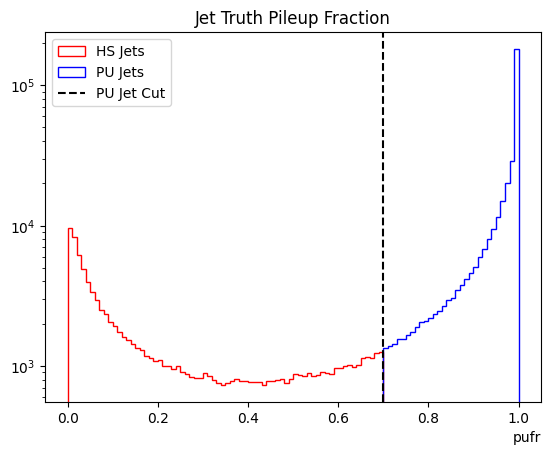
\includegraphics[width=0.3\textwidth]{PU_Jet_Cut}
\caption{An arbitrary cut on the continuous $PU_{fr}$ to recover binary labels.}
\end{figure}

\subsection{Classical JVT Architecture}\hfill

The Jet Vertex Tagger, JVT, was orignally proposed by ATLAS~\cite{ATLAS-CONF-2014-018}. The model uses $R_{pT}$ and corrJVF as input and constructs a likelihood between zero and one which represents the probability in which the jet originated from hard scatter. The JVT model is based on a k-Nearest Neighbor, kNN, algorithm which uses a Euclidean metric in the $R_{pT}$-corrJVF plane and is fit using k=100.

\begin{figure}[h!]
\centering
\begin{subfigure}{.3\textwidth}
  \centering
  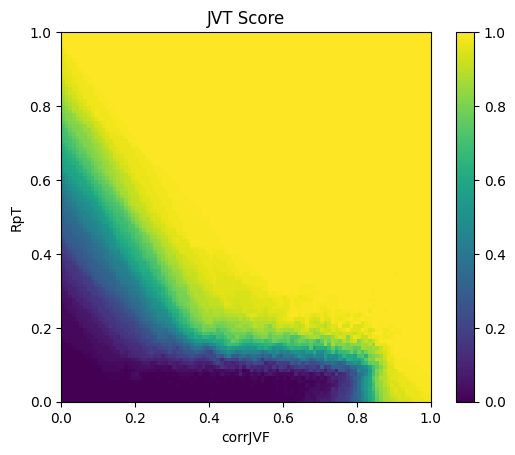
\includegraphics[width=0.9\linewidth]{JVT_2d}
  \caption{}
  \label{fig:sub1}
\end{subfigure}%
\begin{subfigure}{.3\textwidth}
  \centering
  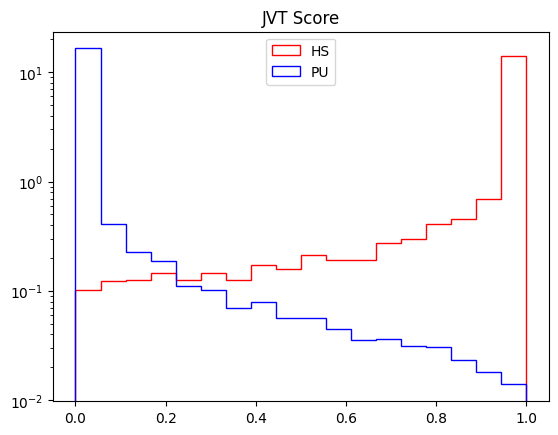
\includegraphics[width=1\linewidth]{JVT_1d}
  \caption{}
  \label{fig:sub2}
\end{subfigure}
\caption{Figure (a) shows JVT liklihood in the $R_{pT}$-corrJVF plane. Figure (b) shows the JVT liklihood for HS and PU jets.}
\label{fig:test}
\end{figure}

\subsection{AttnJVT Architecure}\hfill

To perform a fair benchmark, the orignal JVT model was recreated and performance was evaluated between the original model and the attention model on the same dataset. The input to the model is a unordered set of jets from an event. Each event has a variable number of jets, N, so the input tensor will be of shape $\mathbb{J} \in \mathbb{R}^{N,F}$ where F is the six input features described in section 2.1. The input jets are fed through an initializer, $\phi$, to transform them into the embedding space with dimension D:

\begin{equation}
\phi(\mathbb{J}) \rightarrow \mathbb{E} \in \mathbb{R}^{N,D} 
\end{equation}

The embedded jets are then passed through a multi-head attention layer to update their representations in the context of an entire event. First the embeddings $\mathbb{E}$ are passed through a multi-head attention layer using self attention to generate the context tensor $\mathbb{C}$:

\begin{equation}
\mathbb{C} = MHA(\mathbb{E},\mathbb{E},\mathbb{E})
\end{equation}

Then the context tensor, $\mathbb{C} \in \mathbb{R}^{N,D}$, is concatenated with the original embedding to update the original representation of each jet, $\mathbb{E} = \mathbb{E}+\mathbb{C}$. Lastly, the jet embedding is passed through a final classifier, $\Psi$, to perform binary classification:

\begin{equation}
\Psi(\mathbb{E}) \rightarrow \vec{y} \in \{0,1\}
\end{equation}

The model is trained using the Binary Cross Entropy loss function.

\begin{figure}[h!]
\centering
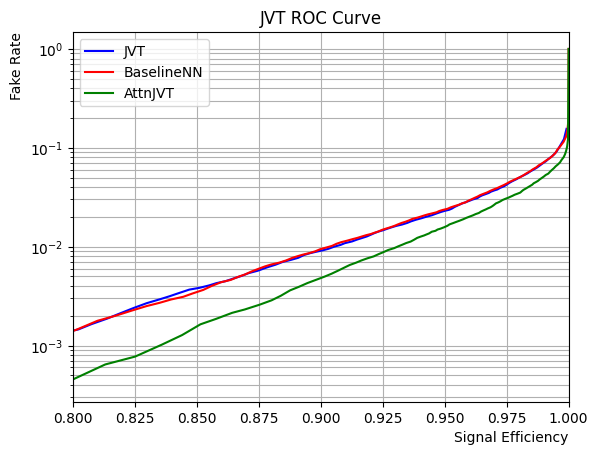
\includegraphics[width=0.5\textwidth]{AttnJVT}
\caption{Using a MHA layer, the jets have access to the context of the entire event which allows the model to capture correlations between HS jets. This effect reduces the fake rate of the model.}
\label{fig:test}
\end{figure}

We benchmarked JVT against AttnJVT to show that we can reduce the fake-rate when we use a Multihead Attention layer which gives jets event context. This event-wide context allows the model to learn correlations between HS jets.

\section{Methodology}\hfill
% Track Tensor, $\mathcal{T}$, in red and Jet Tensor, $\mathcal{J}$, in blue.

We introduce a machine learning approach \myname{} that incorporates jets and tracks to quantify $E_{frac}$ and $M_{frac}$ of jets. We define this problem as a regression task: $f(\mathcal{J},\mathcal{T})[\theta] \Rightarrow M_{frac}$ and $g(\mathcal{J},\mathcal{T})[\psi] \Rightarrow E_{frac}$, where $\theta$ and $\psi$ are model parameters. We consider $\mathcal{J} \in \mathbb{R}^{N_J \times x}$, and $\mathcal{T} \in \mathbb{R}^{N_J \times N_T \times y}$, where $x$ is jet feature dimensions, $y$ is track feature dimensions, $N_J$ is the total number of jets in an event, $N_T$ is the total number of tracks in a given jet. Our aim in this work is to extract rich contextual track information that exists in the jet-track correlation matrix $\mathcal{T}$ to reinforce jet features for the underlying jet-level regression task. We depict the overall architecture of the proposed model in Figure~\ref{fig:Model}.

\begin{figure}[t]
\centering
  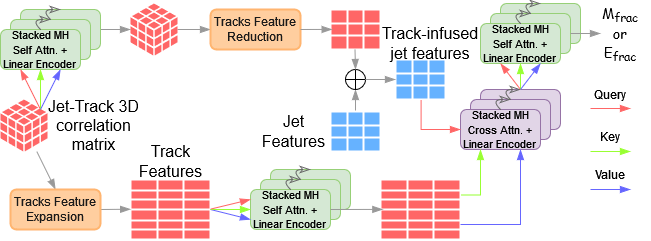
\includegraphics[width=1\linewidth]{PAKDD25-architecture.png}
\caption{Architecture of the proposed attention-based neural network method. Our method extracts two versions of track features to combine with jet features. The proposed multi-head cross-attention block correlates jets with respect to all tracks to enable learning of jet features based on an entire event.}
\label{fig:Model}
\end{figure}

%\rakib{We can say that here $\mathcal{J}$, $\emph{t}$ and $\mathcal{T}$ are jet features, track features independent of jets, and track features associated with jets, respectively.}


%as raw jet features: $[p_T,\eta,\phi,m]$, $\emph{t}$ as raw track features: $[p_T,\eta,\phi,m,d_0,z_0]$\footnote{Transverse, $d_0$, and longitudinal, $z_0$, distance to primary vertex when track is extrapolated to beam line using parameterized estimation}, and $\mathcal{T}$ as a 3d matrix which culminates the entire event with all jet and track features. Therefore, each event can be described by two tensors: a jet tensor $\mathcal{J}\in \mathbb{R}^{N_{J} \times F_{J}}$ and a track tensor $\mathcal{T} \in \mathbb{R}^{N_{J} \times N_{T} \times F_{T}}$ where $N_J$ is the number of jets in the event, $N_T$ is the number of tracks associated to $\mathbb{J}_i$, and $F_{J,T}$ is the number of features for jets and tracks, respectively. Therefore, the goal is to use the architecture in Figure \ref{fig:Model} to approximate the following function, $F(\mathcal{J},\mathcal{T}) \implies [Efrac,Mfrac]$, where Efrac and Mfrac have shape $N_{J}$. \\

% \begin{figure}[h]
% \centering
% \begin{subfigure}{1.0\textwidth}
% \centering
%   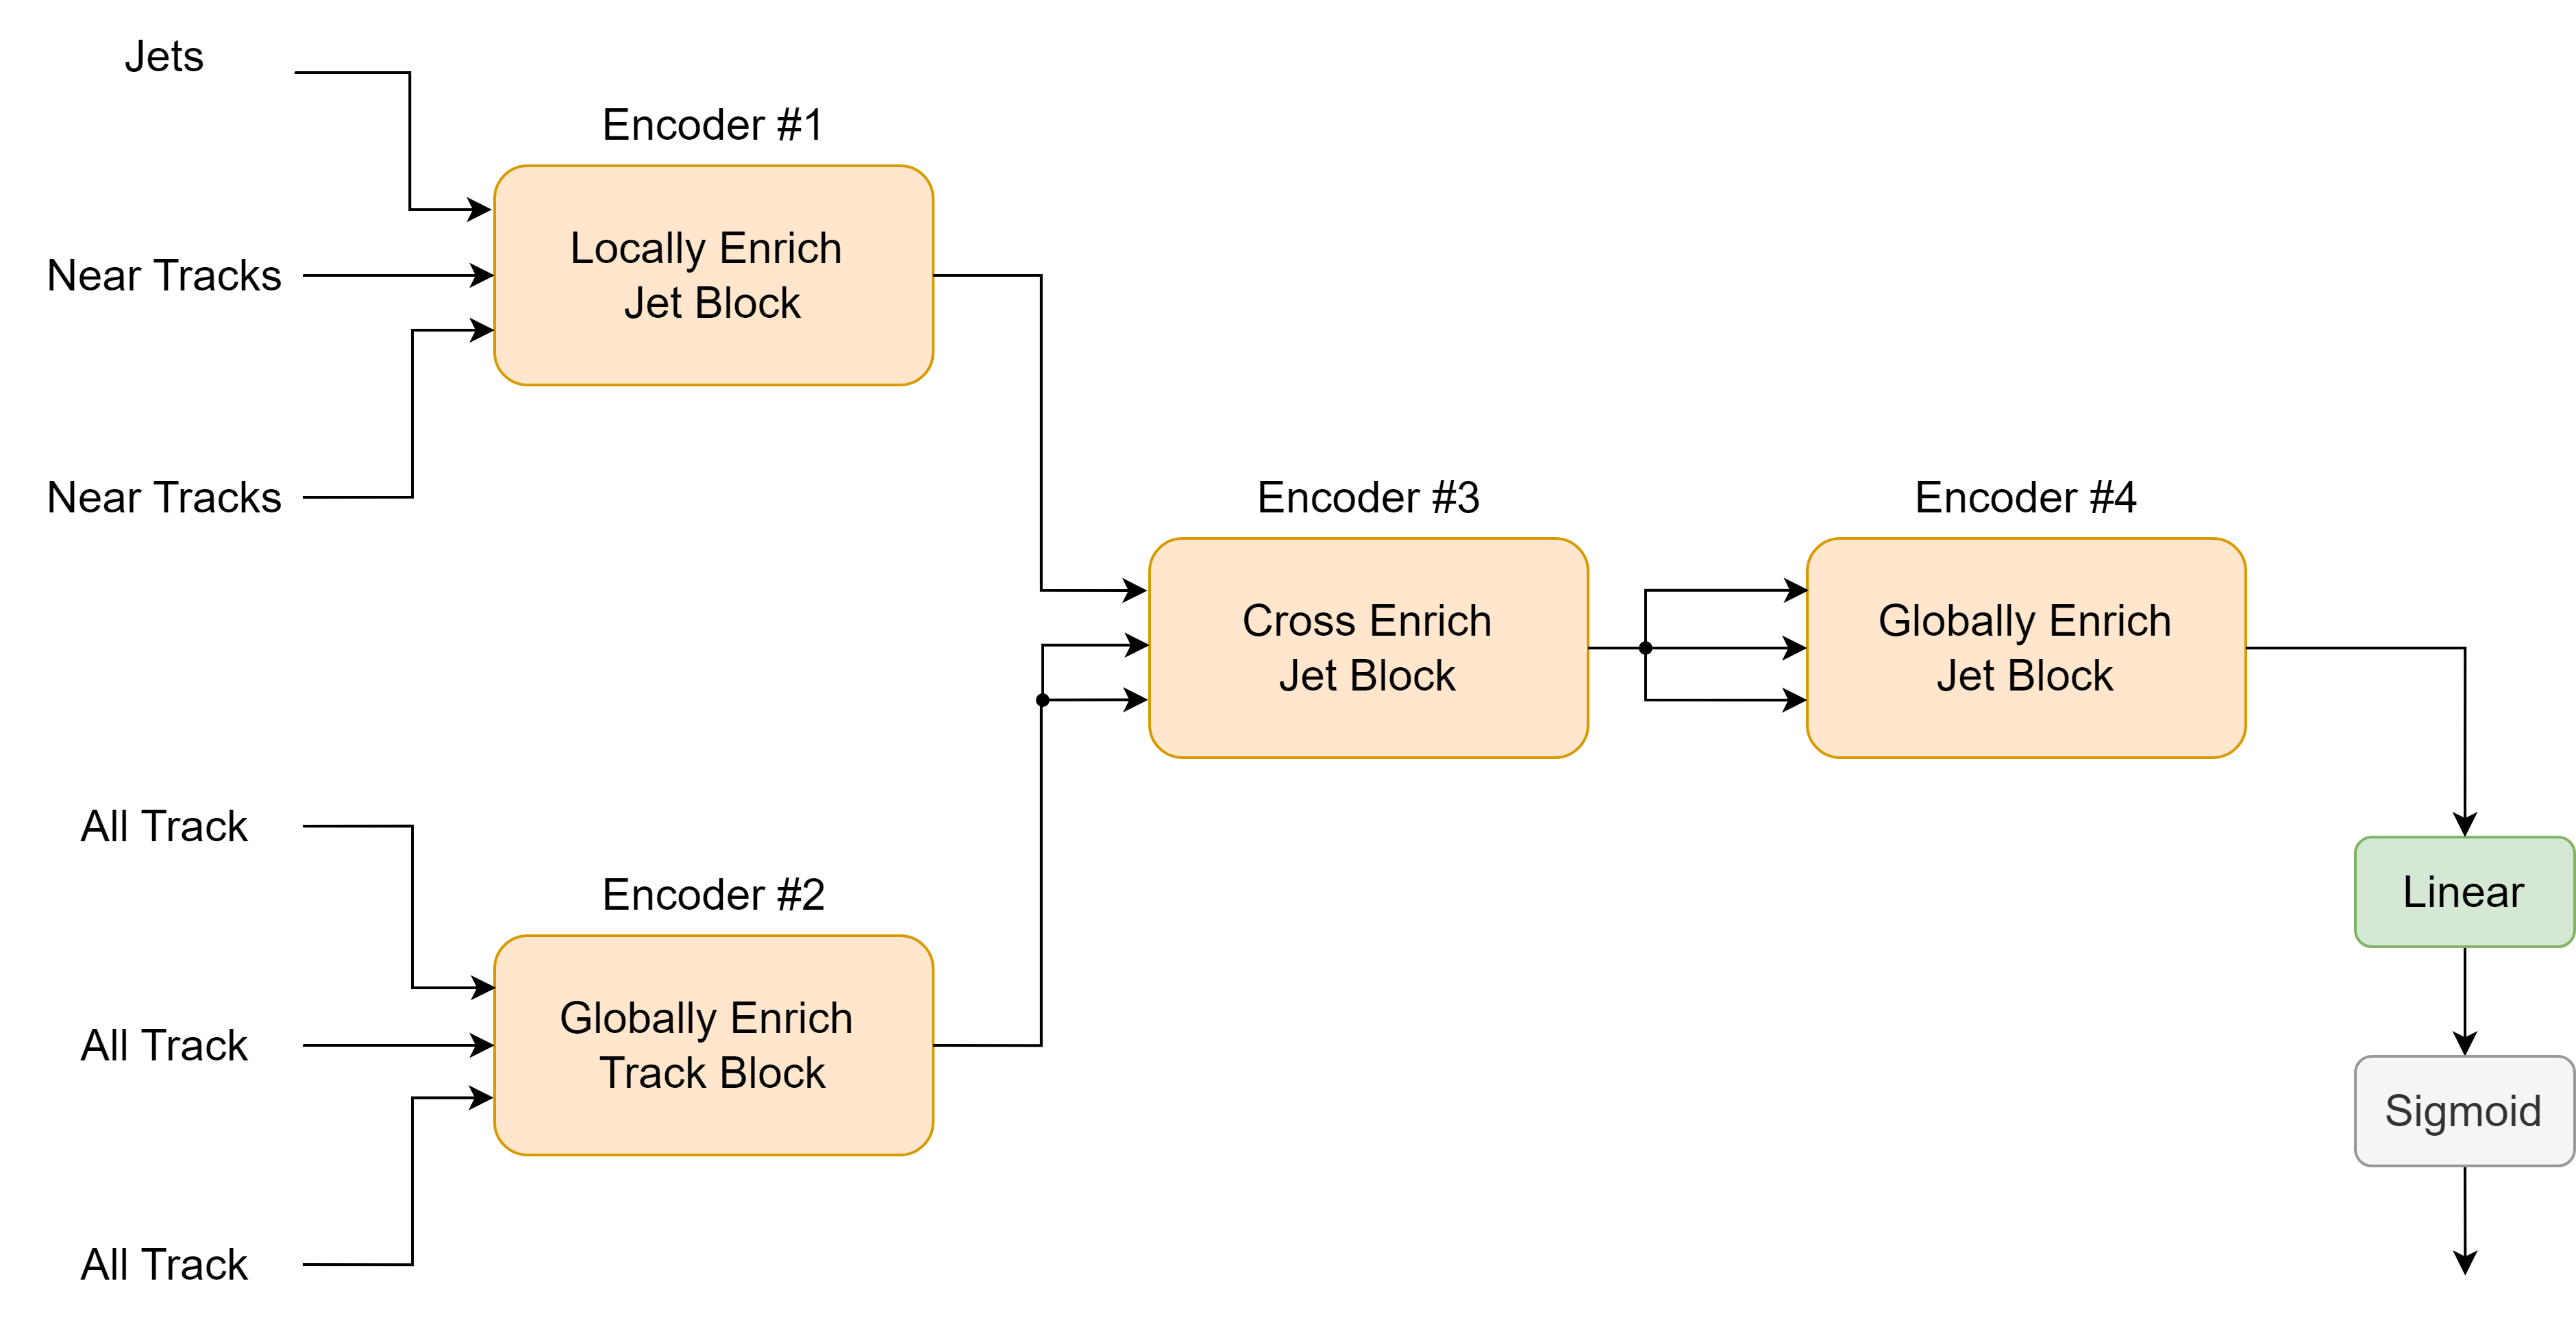
\includegraphics[width=0.70\linewidth]{figures/Physics-PileUp-v1.png}
%   \caption{}
%   \label{fig:sub1}
% \end{subfigure}%
% \hspace{-0.09cm}
% \begin{subfigure}{1.0\textwidth}
%   \centering
%   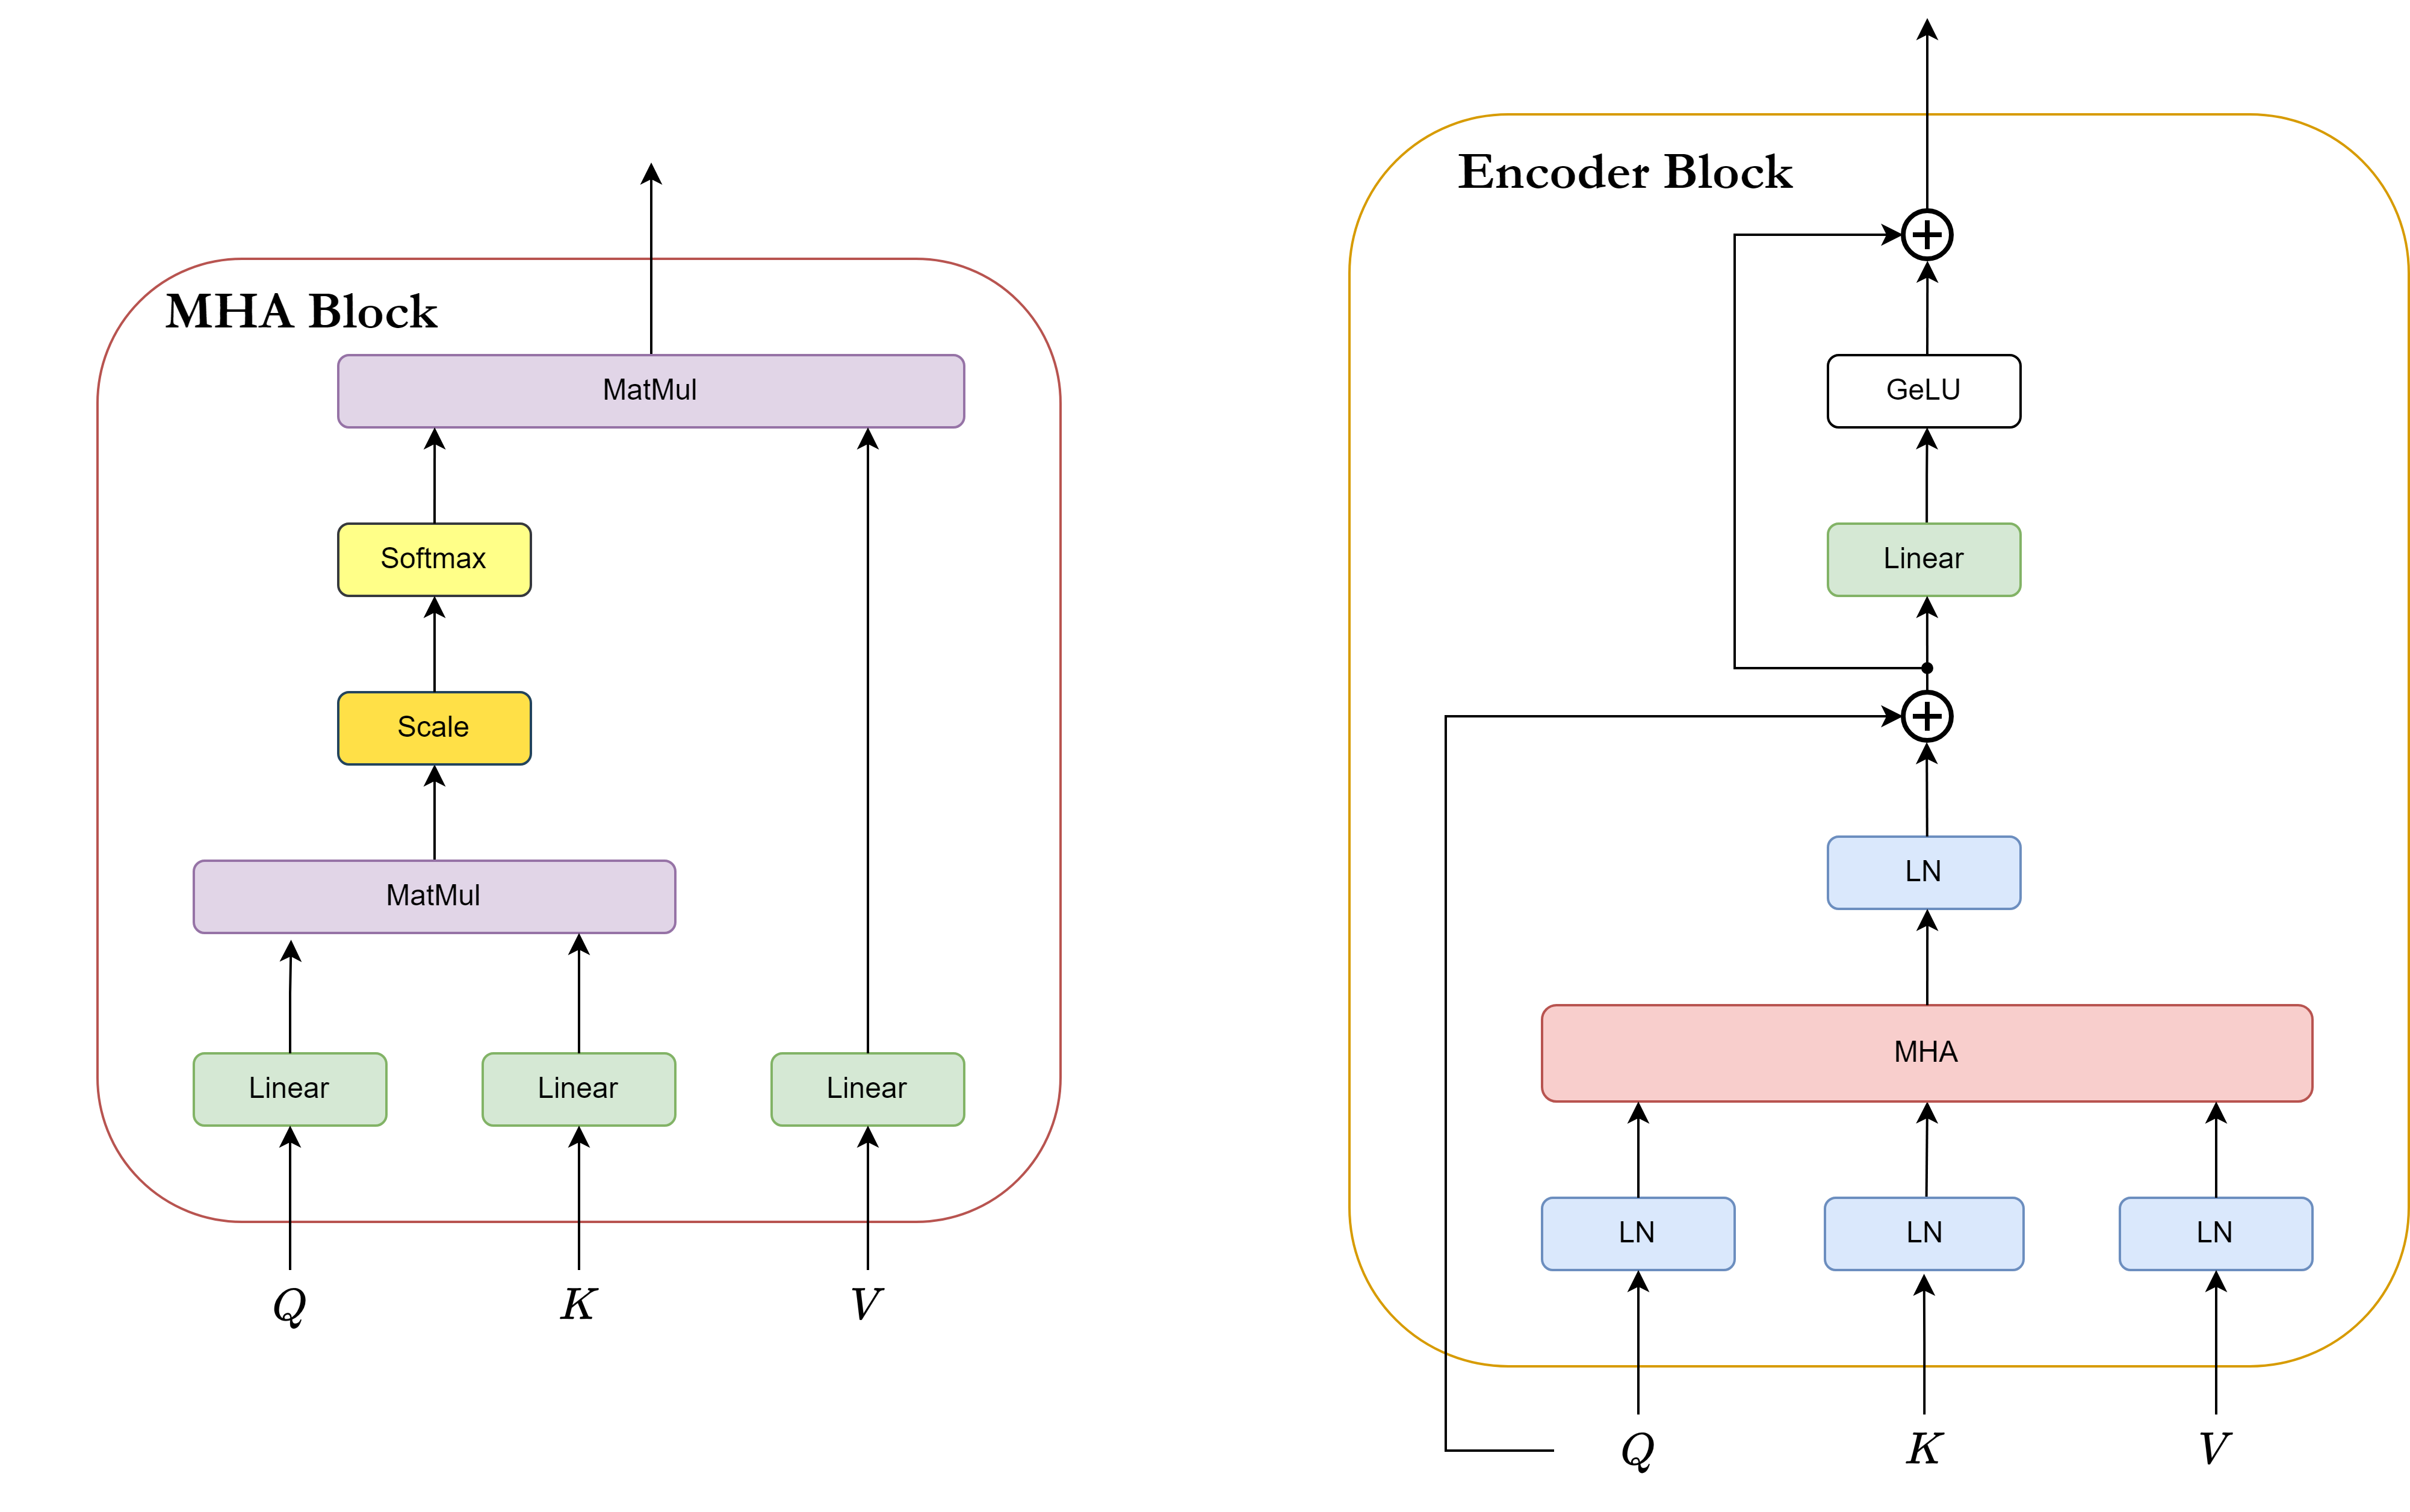
\includegraphics[width=0.70\linewidth]{figures/Physics-PileUp-Encoder-v1.png}
%   \caption{}
%   \label{fig:sub2}
% \end{subfigure}
% \caption{Beautiful Diagram of Model}
% \label{fig:Model}
% \end{figure}



\textbf{Transformer Encoders}: We incorporate encoders with two forms of Set Attention ~\cite{SetAttention} in this work: (i) \emph{Encoders with self-attention} to capture the dependencies of jets and tracks separately, and (ii) \emph{Encoder with cross-attention} to capture the dependencies between jets and tracks on each other. We employ the transformer encoder, which operates on inputs \(Q\) (query), \(K\) (key), and \(V\) (value). First, we apply scaled-dot product attention on normalized vectors to calculate the attention weights and extract correlations: $\text{Attention}(\mathbf{Q}, \mathbf{K}, \mathbf{V}) = \text{softmax}\left(\frac{\mathbf{Q} \mathbf{K}^\top}{\sqrt{d_E}}\right) \mathbf{V}$. We use multi-head attention, $MHA(Q,K,V) = $\\
$ Concat(Attention_1,\ldots,Attention_h)$, where $h$ is the total number of attention heads in the encoder. Second, a residual connections is used to generate the context vector: $\mathbf{Q}_\text{Context} = \mathbf{Q} + \text{MHA}(\mathbf{Q}, \mathbf{K}, \mathbf{V})$. Third, a feed-forward network and an additional skip connection are used to produce the updated representation of the input query: $\mathbf{Q}_\text{Output} = \mathbf{Q}_{\text{Context}} + \text{FFN}(\mathbf{Q}_{\text{Context}})$. This encoder block can be stacked numerous times to iteratively update the query with various key-value pairs. Therefore, the two types of encoders in \myname{} can be represented as given in Equation~\ref{eq:encoders} for inputs $\mathbb{X}$ and $\mathbb{Y}$:

\begin{equation}
    \text{Self-Encoder}(\mathbb{X},\mathbb{X},\mathbb{X}) = \mathbb{X}' \quad \text{Cross-Encoder}(\mathbb{X},\mathbb{Y},\mathbb{Y}) = \mathbb{X}'
    \label{eq:encoders}
\end{equation}

%We first use stacked self attention with linear encoders to learn high-dimensional features of $\emph{t}$ and $\mathcal{T}$.  In particular, we first apply linear transformations on these initial features using three weight parameters $W_q$, $W_k$, and $W_v$ to derive three distinct representations $Q$, $K$, and $V$, respectively, as given below. 

%Our approach leverages a transformer-based encoder to extract contextual representations of jets and tracks by capturing correlations within and between these inputs. The overall architecture of the model is shown in Figure~\ref{fig:Model}.

% \subsection{Transformer Encoder}

% The core building block of our model is a transformer encoder, which operates on inputs \(Q\) (query), \(K\) (key), and \(V\) (value). The encoder consists of the following components:

% 1. Layer Normalization: The inputs are normalized:
% \[
% \mathbf{Q} = \text{LN}(Q), \quad \mathbf{K} = \text{LN}(K), \quad \mathbf{V} = \text{LN}(V),
% \]
% where $\text{LN}(\cdot)$ denotes the layer normalization operation.

% 2. Self-Attention: Relationships between the inputs are computed using scaled dot-product attention:
% \[
% \text{Attention}(\mathbf{Q}, \mathbf{K}, \mathbf{V}) = \text{softmax}\left(\frac{\mathbf{Q} \mathbf{K}^\top}{\sqrt{d_E}}\right) \mathbf{V}.
% \]

% 3. Multi-Head Attention: Multi-head attention splits the embedding dimension \(d_E\) into \(h\) heads for parallel attention computation:
% \[
% \text{MHA}(\mathbf{Q}, \mathbf{K}, \mathbf{V}) = \text{Concat}(\text{head}_1, \ldots, \text{head}_h) \mathbf{W}_o,
% \]
% where $\text{head}_i = \text{Attention}(\mathbf{Q}_i, \mathbf{K}_i, \mathbf{V}_i)$, and $\mathbf{W}_o \in \mathbb{R}^{d_E \times d_E}$ is a learnable output projection matrix.

% 4. Residual Connection: The output of MHA is added back to the query:
% \[
% \text{Context} = \mathbf{Q} + \text{MHA}(\mathbf{Q}, \mathbf{K}, \mathbf{V}).
% \]

% 5. Feed-Forward Network (FFN): The context vector is refined through a feed-forward layer:
% \[
% \text{FFN}(\text{Context}) = \text{GELU}(\text{Context} \mathbf{W}_{\text{ff}} + \mathbf{b}_{\text{ff}}),
% \]
% where $\mathbf{W}_{\text{ff}} \in \mathbb{R}^{d_E \times d_E}$ and $\mathbf{b}_{\text{ff}} \in \mathbb{R}^{d_E}$ are learnable parameters. The final output of the encoder is:
% \[
% \text{Output} = \text{Context} + \text{FFN}(\text{Context}).
% \]

% This encoder is used iteratively in the following sections to process track, jet, and cross-attention features, adapting the query (\(Q\)), key (\(K\)), and value (\(V\)) inputs as per the task.


%\subsection{Feature Embedding}

\textbf{Learning Local Track-reinforced Jet Features $\hat{\mathcal{J}}$}: Apart from using jet features $\mathcal{J}$ for the underlying regression problems $f(\theta)$ and $g(\psi)$, transformer encoders can enrich a jet with its associated tracks for richer jet representations with respect to an event. To aggregate track features in jets, we first correlate jet and track features in the jet-track matrix $\mathcal{T}$ using $\mathcal{T}^{\prime} = \text{Self-Encoder}(\mathcal{T},\mathcal{T},\mathcal{T})$. We then aggregate tracks features of jets $\mathcal{J}_i$ using the sum operation, as given in Equation~\ref{eq:reduction}, where $N_T(\mathcal{J}_i)$ is the number of tracks in the jet $\mathcal{J}_i$. We then align the aggregated jet features $\hat{\mathcal{T}} \in \mathbb{R}^{N_J \times y}$ with the real jet features using the concatenation operation and apply non-linear transformation: $\hat{\mathcal{J}} = \text{ReLU}([\mathcal{J},\hat{\mathcal{T}}]W + b)$, where $W$ and $b$ are trainable weights and biases respectively.

\begin{equation}
\hat{\mathcal{T}}(\mathcal{J}_i) = \sum_{t=1}^{N_T(\mathcal{J}_i)} \mathcal{T}_{t}^{\prime}
\label{eq:reduction}
\end{equation}

\textbf{Learning Global Track Features $t$}: Apart from reinforcing jets with correlations based on local track features, we also aim to enrich jet features independently based on global track correlations during each event. To this end, we first flatten the jet-track correlation matrix $\mathcal{T}$ to consider only the track features $t \in \mathbb{R}^{N_{T} \ \times y}$, where $N_{T}$ is the total number of tracks in the event. We then enrich track features using the stacked self-encoder module: $\hat{t} = \text{Self-Encoder}(t,t,t)$. We emphasize that self-encoder modules on all tracks capture global contextual details in the event. 

\textbf{Learning Global Jet Features}: To model diverse event-wide correlations between jets $\hat{\mathcal{J}}$ and independent tracks $\hat{t}$, we apply encoder with cross-attention as $\mathcal{J}_{\text{cross}} = \text{Cross-Encoder}(\hat{\mathcal{J}},\hat{t},\hat{t})$. These encoded jet representations are based on the global context given by independent track representations that are present both within and outside the jets. Such unique representations allow the model to capture all possible correlations present in hard-scatter processes and give importance to learning jet features at the event-level. We further enrich these jet representations using $\mathcal{J}_{\text{final}} = \text{Self-Encoder}(\mathcal{J}_{\text{cross}},\mathcal{J}_{\text{cross}},\mathcal{J}_{\text{cross}})$.

% the transformer encoder is applied with:
% \[
% Q = \mathcal{J}_{\text{combined}}, \quad K = V = \emph{t}_{\text{embed}}.
% \]
% The output, \(\mathcal{J}_{\text{cross}}\), updates the jet embeddings based on the global context provided by the independent tracks:
% \[
% \mathcal{J}_{\text{cross}} = \text{Encoder}(\mathcal{J}_{\text{combined}}, \emph{t}_{\text{embed}}, \emph{t}_{\text{embed}}).
% \]

% The track aggregation (\ref{sec:trk-agg}) focuses on capturing fine-grained, local track-level details for each jet, while the cross-attention mechanism (\ref{sec:cross}) models global, event-level correlations between jets and independent tracks.

% The input features $\mathcal{J}$, $\emph{t}$, and $\mathcal{T}$ are first embedded into a high-dimensional space of size \(d_E\) using linear transformations followed by ReLU activation:
% \begin{align}
% \mathcal{J}_{\text{embed}} &= \text{ReLU}(\mathcal{J} \mathbf{W}_{\mathcal{J}} + \mathbf{b}_{\mathcal{J}}), \\
% \mathcal{T}_{\text{embed}} &= \text{ReLU}(\mathcal{T} \mathbf{W}_{\mathcal{T}} + \mathbf{b}_{\mathcal{T}}), \\
% \emph{t}_{\text{embed}} &= \text{ReLU}(\emph{t} \mathbf{W}_{\emph{t}} + \mathbf{b}_{\emph{t}}),
% \end{align}
% where $\mathbf{W}_{\mathcal{J}} \in \mathbb{R}^{x \times d_E}$, and \{$\mathbf{W}_{\mathcal{T}}$, $\mathbf{W}_{\emph{t}}$\} $\in$ $\mathbb{R}^{y \times d_E}$ are learnable weight matrices, and $\mathbf{b}_{\mathcal{J}}, \mathbf{b}_{\mathcal{T}}, \mathbf{b}_{\emph{t}} \in \mathbb{R}^{d_E}$ are learnable bias vectors. These embeddings form the initial representations used as inputs to the transformer encoder.


% \subsection{Track Aggregation}
% \label{sec:trk-agg}

% The transformer encoder is applied to the embedded track features (\(\mathcal{T}_{\text{embed}}\)) with:
% \[
% Q = K = V = \mathcal{T}_{\text{embed}}.
% \]
% The encoder output produces updated track embeddings:
% \[
% \mathcal{T}_{\text{updated}} = \text{Encoder}(\mathcal{T}_{\text{embed}}, \mathcal{T}_{\text{embed}}, \mathcal{T}_{\text{embed}}).
% \]
% These embeddings are aggregated across the track dimension for each jet:
% \[
% \hat{\mathcal{T}}_j = \sum_{t=1}^{N_T} \mathcal{T}_{\text{updated}, t}.
% \]

% \subsection{Jet Enrichment}

% The aggregated track embeddings \(\hat{\mathcal{T}}_j\) are concatenated with the jet embeddings \(\mathcal{J}_{\text{embed}}\) and passed through a linear layer followed by ReLU activation to refine the combined representation:
% \[
% \mathcal{J}_{\text{combined}} = \text{ReLU}([\mathcal{J}_{\text{embed}}, \hat{\mathcal{T}}_j] \mathbf{W}_{\text{post}} + \mathbf{b}_{\text{post}}),
% \]
% where \(\mathbf{W}_{\text{post}} \in \mathbb{R}^{2d_E \times d_E}\) and \(\mathbf{b}_{\text{post}} \in \mathbb{R}^{d_E}\). The resulting combined embeddings capture the local track information for each jet, enriched with both jet-level and track-level features.



% % \subsection{Cross-Attention Between Jets and Tracks}
% % \label{sec:cross}

% % To model event-wide correlations between jets and independent tracks (\(\emph{t}\)), the transformer encoder is applied with:
% % \[
% % Q = \mathcal{J}_{\text{combined}}, \quad K = V = \emph{t}_{\text{embed}}.
% % \]
% % The output, \(\mathcal{J}_{\text{cross}}\), updates the jet embeddings based on the global context provided by the independent tracks:
% % \[
% % \mathcal{J}_{\text{cross}} = \text{Encoder}(\mathcal{J}_{\text{combined}}, \emph{t}_{\text{embed}}, \emph{t}_{\text{embed}}).
% % \]

% % The track aggregation (\ref{sec:trk-agg}) focuses on capturing fine-grained, local track-level details for each jet, while the cross-attention mechanism (\ref{sec:cross}) models global, event-level correlations between jets and independent tracks.



% \subsection{Global Jet Contextualization}

% Finally, the enriched jet embeddings \(\mathcal{J}_{\text{cross}}\) are refined using self-attention across all jets:
% \[
% Q = K = V = \mathcal{J}_{\text{cross}}.
% \]
% The encoder output produces the final jet embeddings:
% \[
% \mathcal{J}_{\text{final}} = \text{Encoder}(\mathcal{J}_{\text{cross}}, \mathcal{J}_{\text{cross}}, \mathcal{J}_{\text{cross}}).
% \]

\textbf{Learning Objective}: We predict $E_{frac}$ and $M_{frac}$ using final jet features \(\mathcal{J}_{\text{final}}\) by attaching the regression layer with sigmoid activation function ($\sigma$): $\hat{y} = \sigma(\mathcal{J}_{\text{final}} \mathbf{W}_{\text{out}} + \mathbf{b}_{\text{out}})$, where $\mathbf{W}_{\text{out}}$ and $\mathbf{b}_{\text{out}})$ are learnable regression weights and biases. We optimize all model parameters to learn optimal jet and track features in a supervised fashion using the Mean Squared Error loss function:
\[
\mathcal{L} = \frac{1}{N} \sum_{i=1}^N \left( \hat{y}_i - y_i \right)^2,
\]
where \(N\) is the total number of training samples, $y$ is the ground truth ($E_{frac}$ or $M_{frac}$), and $\hat{y}$ is the model prediction. By leveraging track features and global context through iterative encoder-based attention mechanisms, the model progressively refines jet features to predict energy and mass fractions with least mean square error.


% \subsection{Regression}

% The final jet embeddings, \(\mathcal{J}_{\text{final}}\), are passed through a regression layer with sigmoid activation to predict \(E_{\text{frac}}\) and \(M_{\text{frac}} \):
% \[
% \hat{y} = \sigma(\mathcal{J}_{\text{final}} \mathbf{W}_{\text{out}} + \mathbf{b}_{\text{out}}),
% \]
% where \(\mathbf{W}_{\text{out}} \in \mathbb{R}^{d_E \times 1}\) and \(\mathbf{b}_{\text{out}} \in \mathbb{R}\). This layer maps the enriched jet embeddings to the desired output space, producing predictions for the energy and mass fractions.

% \subsection{Learning Objective}

% The model is trained using the mean squared error (MSE) loss, which minimizes the difference between the predicted values, \(\hat{y}\), and the ground truth labels, \(y\):
% \[
% \mathcal{L} = \frac{1}{N} \sum_{i=1}^N \left( \hat{y}_i - y_i \right)^2,
% \]
% where \(N\) is the total number of training samples.

% By leveraging track features and global context through iterative encoder-based attention mechanisms, the model progressively refines jet embeddings to predict energy and mass fractions with high accuracy.


% We use multihead self attention~\cite{Attention} to learn attention weights of tracks and jet-tracks which are then combined with values to derive contextual representations. We further use linear layer and a feed forward neural network to obtain , as given in the following equations, which captures inherent semantically important information present within $\emph{t}$ correlations and $\mathcal{T}$ correlations respectively.  

% \arun{multihead and NN equations go here}

%overall model architecture can be considered a stack of various transformer encoders using multi-head attention~\cite{Attention} to approximate the optimal high-dimensional embedding of jets in the context of an event. Since a jet itself is only described by four features, various transformer encoders use self attention to capture track-track and jet-jet correlations and cross attention to capture jet-track correlations which heavily enriches the embedded representation of a jet. 

% Effectively, apart from using jet features for the underlying regression problems $f(\theta)$ and $g(\psi)$, transformer encoders can enrich a jet with its associated tracks and all other possible information from the event allowing for a richer embedded representation. It is with these enriched jet embeddings that the model is able to learn, from data, the hard scatter energy and mass fractions of each jet in an event.

% \begin{equation}
%     \hat{\mathcal{T}}_j = \sum_{t=1}^{|\mathcal{T}_J|} \mathcal{T}_{jt}
% \end{equation}

% In real-world experiments, jet features can be largely aligned with tracks associated with them. We combine jet features with track features that are reduced from jet-track features using a linear operation such as concatenation: $\mathcal{J} = \mathcal{J} \oplus \hat{\mathcal{T}}$.

% With context enriched jet features and track features, it is necessary to understand correlations of jets, not only with tracks within, but also with tracks outside them. We employ cross-encoder module, as given in Equation , to learn these diverse correlations between jets and tracks. This cross encoder module allows jets to update their representations with tracks outside their cone, which allows the model to capture all possible correlations present in hard-scatter processes.

% \arun{Cross attention block goes here}

% \arun{Learning objective}

%\luke{vvvvvv  This paragraph is bad but I am trying to explain the encoders}\\
%Each encoder block uses a Query and Key-Value pair to enrich a set of queries in the context of a set of keys. Due to the inherent unordered nature of sets, no position encoding is required. Scaled dot product attention is used to generate attention weights, an $N \times M$ matrix, where $N$ and $M$ are the cardinality of the query and key sets, respectively. These attention weights allow the model to learn correlations between elements of the query and key set which is fundamentally required to extract the hard scatter correlations present in the dataset. Layer normalizations are used to stabilize the training process REF [NORMFORMER]. The output of the MHA block can be interpreted as a \emph{context} vector that can be added element wise to the query through a skip connection. This combined vector is passed through a linear layer with GeLU activation and another skip connection is applied to deliver the updated representation of the query set in the context of the key set. \\

% Tensors $\mathcal{J}$ and $\mathcal{T}$ are first processed using linear layer with GeLU activation to transform from the feature space to an initial embedding space, $F_{J,T} \rightarrow d_E$. Then two types of encoders are used:
% \begin{equation}
%   \text{Self-Encoder}(\mathbb{X},\mathbb{X},\mathbb{X})=\mathbb{X}' \phantom{.......} \text{Cross-Encoder}(\mathbb{X},\mathbb{Y},\mathbb{Y})=\mathbb{X}'
% \end{equation}
%where $\mathbb{X}$ and $\mathbb{Y}$ are sets representing Query, Key, and Value. First, jets are enriched using their associated tracks using the "Locally Enrich Jet Encoder Block". 

% This is done by: $\text{Self-Encoder}(\mathcal{T},\mathcal{T},\mathcal{T})=\mathcal{T}'$, reduction operation over $N_T$ dimension, then concatenated with the $\mathcal{J}$ tensor along $d_E$ dimension to form tensor $\mathcal{J}'$. Second, tracks are enriched at the event level by flattening along $N_T$ dimension to form $\mathcal{T}_{flat}$, and passed through "Globally Enrich Track Block", $\text{Self-Encoder}(\mathcal{T}_{flat},\mathcal{T}_{flat},\mathcal{T}_{flat})=\mathcal{T}_{flat}'$. This block allows hard scatter tracks to pass information throughout the entire event. Third, the novel "Cross Enrich Jet Block" uses $\text{Cross-Encoder}(\mathcal{J}',\mathcal{T}_{flat}',\mathcal{T}_{flat}')=\mathcal{J}''$. This cross encoder block allows jets to update their representations with tracks outside their cone, which allows the model to capture all possible correlations present in hard scatter processes. Fourth and finally, the "Globally Enrich Jet Encoder Block" is used to update jets in the context of an entire event, $\text{Self-Encoder}(\mathcal{J}'',\mathcal{J}'',\mathcal{J}'')=\mathcal{J}_{Event}$. This tensor, $\mathcal{J}_{Event}$, represents the high dimensional embeddings of the jets in the event, and can be used to quantify the amount of pileup, Efrac and Mfrac, using a final regression layer with sigmoid activation. \\

% The model is trained on the diHiggs simulated dataset, described in Section \ref{Dataset} depicted in Figure \ref{fig:HLLHC}, using Efrac and Mfrac as targets, described in Section \ref{JetLabels} depicted in Figure \ref{fig:Labels}. In practice, each encoder block is duplicated 3 times to give the model more learnable parameters, $\sim$4.1M,  to achieve a deeper representation of jets. During the training process, the learning rate is scheduled to decay by a factor of 0.1 after the 25th epoch which noticeably helped descend the noisy loss landscape. The AdamW optimizer is used to prevent overtraining using weight decay, and Mean Squared Error was used as the loss function. The model converged after training 50 epochs on an NVIDIA RTX 3090.


%The model is trained on the diHiggs simulated dataset, described in Section \ref{Dataset} depicted in Figure \ref{fig:HLLHC}, using Efrac and Mfrac as targets, described in Section \ref{JetLabels} depicted in Figure \ref{fig:Labels} using a Mean Squared Error loss function.



%%%%%%%%%%%%%%%%%%%%%%%%%%
%%% Multi-Line Comment %%%
%%%%%%%%%%%%%%%%%%%%%%%%%%
\iffalse
\subsection{Model Architecture}\hfill

Four transformer encoder stacks are used to enrich each tensor -- $\mathbb{J},\mathbb{T}_{jet},\mathbb{T}_{jet}$ -- with context from the event. Each encoder follows the NormFormer [*] architecture by (... et al). NormFormers consists of LayerNorms, LN(), multi-head attention, MHA(), skip connections, + operator, feed-forward network, FFN, which consists of a linear layer and a GELU activation function. These layers are the components of each encoder block.


First, each jet is enriched with associated tracks. Since each jet only carries four features, $p_T, \eta, \phi, m$, tracks within a radius of $\Delta R = 0.4$ are used in the first encoder stack to achieve a rich representation of each jet.

\begin{align}
    \mathbb{T}_{context} &= \mathbb{T}_{jet} + LN(MHA(LN(\mathbb{T}_{jet}), LN(\mathbb{T}_{jet}), LN(\mathbb{T}_{jet}))) \\
    \mathbb{T}_{embed} &= \mathbb{T}_{context} + FFN (\mathbb{T}_{context}) \\
    \mathbb{T}_{aggregated} &= \sum_{dim=1} \mathbb{T}_{embed} \\ 
    \mathbb{J}_{enriched} &= FFN(\mathbb{J} \mathop{\oplus}_{dim=1} \mathbb{T}_{aggregated})
\end{align}
$\mathbb{T}_{jet}$, $\mathbb{T}_{context}$, and $\mathbb{T}_{embed}$ all have shape $N_{jet} \times N_{trk} \times E_{dim}$. Then the summation operator reduces the $N_{trk}$ dimension which will then match the dimension of $\mathbb{J}$ with shape $N_{jet} \times E_{dim}$. The jet and aggregated track tensors are concatenated along the embedding dimension, and the FFN has input $N_{jet} \times 2\cdot E_{dim}$ and outputs $\mathbb{J}$ of shape $N_{jet} \times E_{dim}$. This encoder block can be interpreted physically as learning to enrich the jet in the context of associated particles. %For example, if there is are particles that resemble b-hadron decay, this encoder block might enrich this jet as a b-jet in the latent space.

Second, $\mathbb{T}_{event}$ with shape $N_{trk} \times E_{dim}$ are enriched using an encoder block using self-attention:
\begin{align}
    \mathbb{T}_{context} &= \mathbb{T}_{event} + LN(MHA(LN(\mathbb{T}_{event}), LN(\mathbb{T}_{event}), LN(\mathbb{T}_{event}))) \\
    \mathbb{T}_{embed} &= \mathbb{T}_{context} + FFN (\mathbb{T}_{context})
\end{align}
The purpose of this encoder is to update all tracks in the context of the event and initialize them for cross attention with jets.

Third, cross attention between $\mathbb{J}_{enriched}$ and $\mathbb{T}_{embed}$ is performed to update the jets in the context of all tracks of the event.

\begin{align}
    \mathbb{J}_{context} &= \mathbb{J}_{enriched} + LN(MHA(LN(\mathbb{J}_{enriched}), LN(\mathbb{T}_{event}), LN(\mathbb{T}_{event}))) \\
    \mathbb{J}_{embed} &= \mathbb{J}_{context} + FFN (\mathbb{J}_{context})
\end{align}

%This encoder allows tracks to update the jet embedding in the context of an event. For example, if we consier $t \rightarrow Wb \rightarrow l\nu b$, this encoder allows the high energy lepton, l, to update the context of the b-jet.

Fourth and finally, $\mathbb{J}_{embed}$ with shape $N_{jet} \times E_{dim}$ is enriched using a encoder block using self attention:

\begin{align}
    \mathbb{J}_{context} &= \mathbb{J}_{embed} + LN(MHA(LN(\mathbb{J}_{embed}), LN(\mathbb{J}_{embed}), LN(\mathbb{J}_{embed}))) \\
    \mathbb{J}_{embed} &= \mathbb{J}_{context} + FFN (\mathbb{J}_{context})
\end{align}

This encoder is performed last because at this stage the jets have achieved a rich representation after passing through the previous encoders. This last encoder allows jets to update their representation in the context of an event. This encoder can be interpreted physically as allowing jets to update representations according to conservation of momentum or other properties that might be shared between jets.

Lastly, the embedded jet vectors are passed through a final classification layer to predict the continuous Efrac and Mfrac label.
\fi
%%%%%%%%%%%%%%%%%%%%%%%%%%
%%% Multi-Line Comment %%%
%%%%%%%%%%%%%%%%%%%%%%%%%%


%\hfill\\
\section{Methodology}\hfill

In this work, we introduce a machine learning approach that incorporates jets and tracks to quantify $E_{frac}$ and $M_{frac}$ of jets. We define this problem as a regression task: $f(\mathcal{J},\mathcal{T})[\theta] \Rightarrow M_{frac}$ and $g(\mathcal{J},\mathcal{T})[\psi] \Rightarrow E_{frac}$, where $\theta$ and $\psi$ are model parameters. We consider jet tensor $\mathcal{J} \in \mathbb{R}^{N_J \times x}$ with features: $[p_T,\eta,\phi,m]$, and track tensor $\mathcal{T} \in \mathbb{R}^{N_J \times N_T \times y}$ with features: $[p_T,\eta,\phi,m,d_0,z_0]$\footnote{Transverse, $d_0$, and longitudinal, $z_0$, distance to primary vertex when track is extrapolated to beam line using parameterized estimation}, where $x$ is jet feature dimensions, $y$ is track feature dimensions, $N_J$ is the total number of jets in an event, $N_T$ is the total number of tracks in an event. We depict the overall architecture of the proposed model in Figure~\ref{fig:Model}. The goal of this work is to extract rich contextual information that exists in track features, $\mathcal{T}$, to reinforce jet features, $\mathcal{J}$, using transformer-based encoder to capture correlations within and between these inputs.

\begin{figure}[h]
\centering
  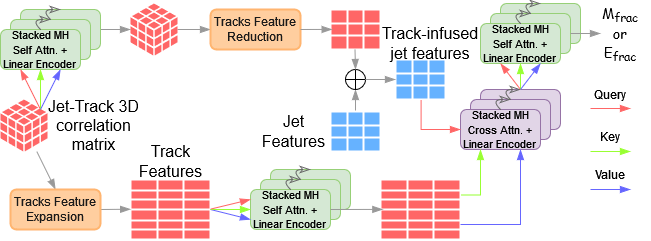
\includegraphics[width=1\linewidth]{PAKDD25-architecture.png}
\caption{Track Tensor, $\mathcal{T}$, in red and Jet Tensor, $\mathcal{J}$, in blue.}
\label{fig:Model}
\end{figure}


\subsection{Transformer Encoder} \hfill

The core building block of our model is a transformer encoder, which operates on inputs \(Q\) (query), \(K\) (key), and \(V\) (value). First, the encoder uses Layer Normalization to initialize inputs: $\mathbf{Q} = \text{LN}(Q), \mathbf{K} = \text{LN}(K), \mathbf{V} = \text{LN}(V)$. Second, scaled-dot product attention is used to calculate the attention weights and extract correlations: $\text{Attention}(\mathbf{Q}, \mathbf{K}, \mathbf{V}) = \text{softmax}\left(\frac{\mathbf{Q} \mathbf{K}^\top}{\sqrt{d_E}}\right) \mathbf{V}$. In practice, multi-head attention, MHA, is used for deeper learning where $num\_heads=8$. Third, a residual connections is used to generate the context vector: $\mathbf{Q}_\text{Context} = \mathbf{Q} + \text{MHA}(\mathbf{Q}, \mathbf{K}, \mathbf{V})$. Fourth, a feed-forward network and additional skip connection is used to produce the updated representation of the input query: $\mathbf{Q}_\text{Output} = \mathbf{Q}_\text{Context} + \text{FFN}(\mathbf{Q}\text{Context})$. This encoder block can be stacked numerous times to iteratively update the query with various key-value pairs. Therefore, the two types of encoder used by the model can be summarized as self-encoders and cross-encoders for input sets $\mathbb{X}$ and $\mathbb{Y}$:

\begin{equation}
    \text{Self-Encoder}(\mathbb{X},\mathbb{X},\mathbb{X}) = \mathbb{X}' \quad \text{Cross-Encoder}(\mathbb{X},\mathbb{Y},\mathbb{Y}) = \mathbb{X}'
\end{equation}

\subsection{Local Track Enrichment of Jets}
\label{sec:trk-agg}

The first method to enrich $\mathcal{J}$ with $\mathcal{T}$ is depicted in the upper branch of Figure \ref{fig:Model} through a 3-step process: (1) self-encoder is applied to $\mathcal{T}$ to capture local correlations between tracks, (2) reduction operation is applied, and (3) reduced track tensor is concatenated with jet tensor to achieve an updated representation of jets. These operatoins are summarized as:

\begin{align}
  \mathcal{T}' &= \text{Self-Encoder}(\mathcal{T},\mathcal{T},\mathcal{T}) \\
  \mathcal{T}_\text{reduced}&=\sum\limits_{dim=1} \mathcal{T}' \\
  \mathcal{J}_\text{local}&=\mathcal{J} \oplus \mathcal{T}_\text{reduced}
\end{align}


\subsection{Global Track Enrichment of Jets} \hfill

The second method to enrich $\mathcal{J}$ with $\mathcal{T}$ is depicted in the lower branch of Figure \ref{fig:Model} through a 3-step process: (1) feature expansion is applied to flatten $\mathcal{T}$, (2) self-encoder is applied to $\mathcal{T}$ to capture global correlations between tracks, and (3) cross-encoder is applied to $\mathcal{J}$ and $\mathcal{T}$ to capture correlations between jets and all tracks.

\begin{align}
  \mathcal{T}_\text{flat}&=\text{Flatten}(\mathcal{T},dim=1) \\
  \mathcal{T}_\text{flat}' &= \text{Self-Encoder}(\mathcal{T}_\text{flat},\mathcal{T}_\text{flat},\mathcal{T}_\text{flat}) \\
  \mathcal{J}_\text{global} &= \text{Cross-Encoder}(\mathcal{J}_\text{local},\mathcal{T}_\text{flat}',\mathcal{T}_\text{flat}') \\
\end{align}

A final self-encoder between jets is used to provide full event context: $\mathcal{J}_\text{final} = \text{Self-Encoder}(\mathcal{J}_\text{global},\mathcal{J}_\text{global},\mathcal{J}_\text{global}) $. These final jet embeddings, \(\mathcal{J}_{\text{final}}\), are passed through a regression layer with sigmoid activation to predict $E_{\text{frac}}$ and $M_{\text{frac}}$.

\subsection{Learning Objective}\hfill

The model is trained on the diHiggs simulated dataset, described in Section \ref{Dataset} depicted in Figure \ref{fig:HLLHC}, using Efrac and Mfrac as targets, described in Section \ref{JetLabels} depicted in Figure \ref{fig:Labels} using a Mean Squared Error loss function. In practice, each encoder block is stacked three times to give the model more learnable parameters, $\sim$4.1M,  to achieve a deeper representation of jets. During the training process, the learning rate is scheduled to decay by a factor of 0.1 after the 25th epoch which noticeably helped descend the noisy loss landscape. The AdamW optimizer is used to prevent overtraining using weight decay, and Mean Squared Error was used as the loss function. The model converged after training 50 epochs on an NVIDIA RTX 3090.


%%%%%%%%%%%%%%%%%%%%%%%%%%
%%% Multi-Line Comment %%%
%%%%%%%%%%%%%%%%%%%%%%%%%%
\iffalse
\subsection{Model Architecture}\hfill

Four transformer encoder stacks are used to enrich each tensor -- $\mathbb{J},\mathbb{T}_{jet},\mathbb{T}_{jet}$ -- with context from the event. Each encoder follows the NormFormer [*] architecture by (... et al). NormFormers consists of LayerNorms, LN(), multi-head attention, MHA(), skip connections, + operator, feed-forward network, FFN, which consists of a linear layer and a GELU activation function. These layers are the components of each encoder block.


First, each jet is enriched with associated tracks. Since each jet only carries four features, $p_T, \eta, \phi, m$, tracks within a radius of $\Delta R = 0.4$ are used in the first encoder stack to achieve a rich representation of each jet.

\begin{align}
    \mathbb{T}_{context} &= \mathbb{T}_{jet} + LN(MHA(LN(\mathbb{T}_{jet}), LN(\mathbb{T}_{jet}), LN(\mathbb{T}_{jet}))) \\
    \mathbb{T}_{embed} &= \mathbb{T}_{context} + FFN (\mathbb{T}_{context}) \\
    \mathbb{T}_{aggregated} &= \sum_{dim=1} \mathbb{T}_{embed} \\ 
    \mathbb{J}_{enriched} &= FFN(\mathbb{J} \mathop{\oplus}_{dim=1} \mathbb{T}_{aggregated})
\end{align}
$\mathbb{T}_{jet}$, $\mathbb{T}_{context}$, and $\mathbb{T}_{embed}$ all have shape $N_{jet} \times N_{trk} \times E_{dim}$. Then the summation operator reduces the $N_{trk}$ dimension which will then match the dimension of $\mathbb{J}$ with shape $N_{jet} \times E_{dim}$. The jet and aggregated track tensors are concatenated along the embedding dimension, and the FFN has input $N_{jet} \times 2\cdot E_{dim}$ and outputs $\mathbb{J}$ of shape $N_{jet} \times E_{dim}$. This encoder block can be interpreted physically as learning to enrich the jet in the context of associated particles. %For example, if there is are particles that resemble b-hadron decay, this encoder block might enrich this jet as a b-jet in the latent space.

Second, $\mathbb{T}_{event}$ with shape $N_{trk} \times E_{dim}$ are enriched using an encoder block using self-attention:
\begin{align}
    \mathbb{T}_{context} &= \mathbb{T}_{event} + LN(MHA(LN(\mathbb{T}_{event}), LN(\mathbb{T}_{event}), LN(\mathbb{T}_{event}))) \\
    \mathbb{T}_{embed} &= \mathbb{T}_{context} + FFN (\mathbb{T}_{context})
\end{align}
The purpose of this encoder is to update all tracks in the context of the event and initialize them for cross attention with jets.

Third, cross attention between $\mathbb{J}_{enriched}$ and $\mathbb{T}_{embed}$ is performed to update the jets in the context of all tracks of the event.

\begin{align}
    \mathbb{J}_{context} &= \mathbb{J}_{enriched} + LN(MHA(LN(\mathbb{J}_{enriched}), LN(\mathbb{T}_{event}), LN(\mathbb{T}_{event}))) \\
    \mathbb{J}_{embed} &= \mathbb{J}_{context} + FFN (\mathbb{J}_{context})
\end{align}

%This encoder allows tracks to update the jet embedding in the context of an event. For example, if we consier $t \rightarrow Wb \rightarrow l\nu b$, this encoder allows the high energy lepton, l, to update the context of the b-jet.

Fourth and finally, $\mathbb{J}_{embed}$ with shape $N_{jet} \times E_{dim}$ is enriched using a encoder block using self attention:

\begin{align}
    \mathbb{J}_{context} &= \mathbb{J}_{embed} + LN(MHA(LN(\mathbb{J}_{embed}), LN(\mathbb{J}_{embed}), LN(\mathbb{J}_{embed}))) \\
    \mathbb{J}_{embed} &= \mathbb{J}_{context} + FFN (\mathbb{J}_{context})
\end{align}

This encoder is performed last because at this stage the jets have achieved a rich representation after passing through the previous encoders. This last encoder allows jets to update their representation in the context of an event. This encoder can be interpreted physically as allowing jets to update representations according to conservation of momentum or other properties that might be shared between jets.

Lastly, the embedded jet vectors are passed through a final classification layer to predict the continuous Efrac and Mfrac label.
\fi
%%%%%%%%%%%%%%%%%%%%%%%%%%
%%% Multi-Line Comment %%%
%%%%%%%%%%%%%%%%%%%%%%%%%%


\section{Experiments and Results}\hfill

\textbf{\myname{} Setup:} We deploy \myname{} with each encoder block stacked three times to achieve a deeper representation of jets. We schedule the learning rate to decay by a factor of 0.1 after the $25^{th}$ epoch which noticeably helped descend the noisy loss landscape in model training. The \emph{AdamW} optimizer is used to prevent overtraining using weight decay and we use $R^2$ as an evaluation metric. The model converged after training 50 epochs on an NVIDIA RTX 3090.\\

\begin{figure}[ht!]
\begin{subfigure}{.25\textwidth}
  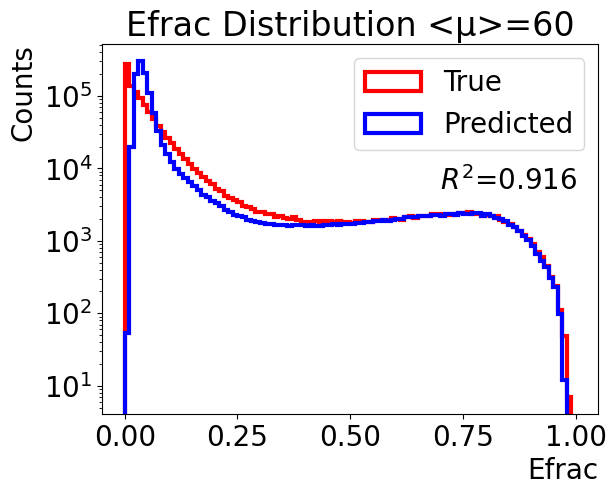
\includegraphics[width=1\linewidth]{Efrac1D_mu60.png}
  \caption{}
  \label{fig:Efrac1d_mu60}
\end{subfigure}%
\begin{subfigure}{.25\textwidth}
  \includegraphics[width=1\linewidth]{Efrac2d_mu60.png}
  \caption{}
  \label{fig:Efrac2d_mu60}
\end{subfigure}
\begin{subfigure}{.25\textwidth}
  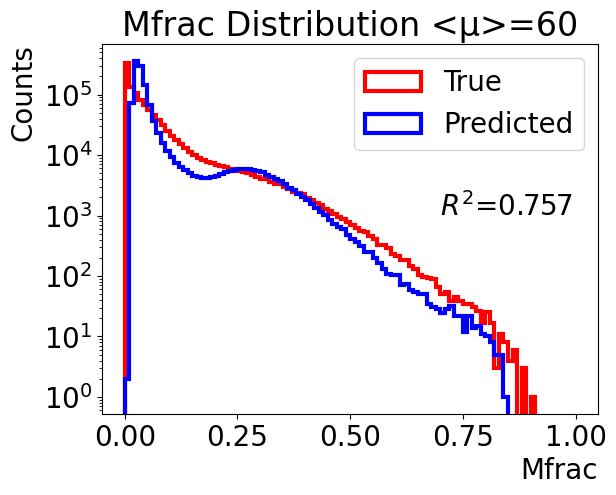
\includegraphics[width=1\linewidth]{Mfrac1D_mu60.png}
  \caption{}
  \label{fig:Mfrac1d_mu60}
\end{subfigure}%
\begin{subfigure}{.25\textwidth}
  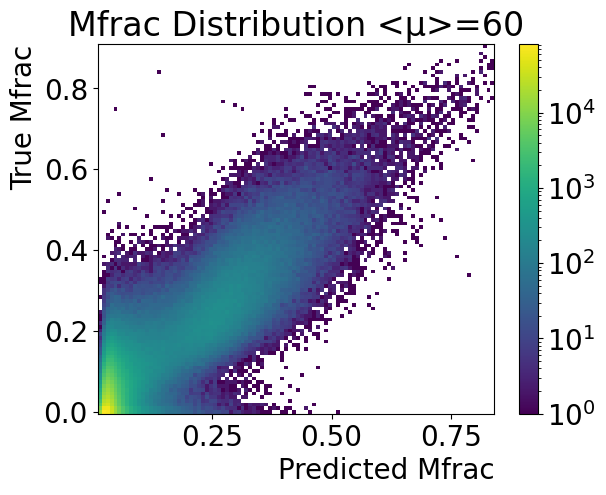
\includegraphics[width=1\linewidth]{Mfrac2D_mu60.png}
  \caption{}
  \label{fig:Mfrac2d_mu60}
\end{subfigure}
\begin{subfigure}{.25\textwidth}
  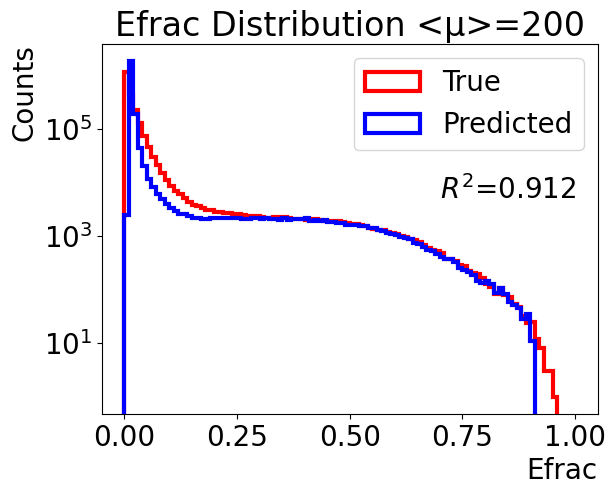
\includegraphics[width=1\linewidth]{Efrac1D_mu200.png}
  \caption{}
  \label{fig:Efrac1d_mu200}
\end{subfigure}%
\begin{subfigure}{.25\textwidth}
  \includegraphics[width=1\linewidth]{Efrac2d_mu200.png}
  \caption{}
  \label{fig:Efrac2d_mu200}
\end{subfigure}
\begin{subfigure}{.25\textwidth}
  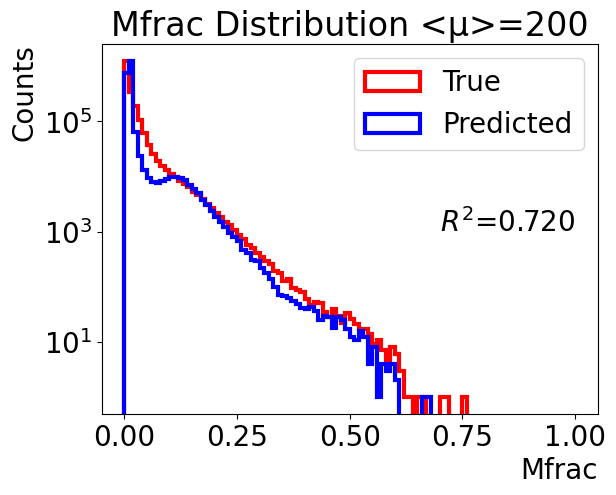
\includegraphics[width=1\linewidth]{Mfrac1D_mu200.png}
  \caption{}
  \label{fig:Mfrac1d_mu200}
\end{subfigure}%
\begin{subfigure}{.25\textwidth}
  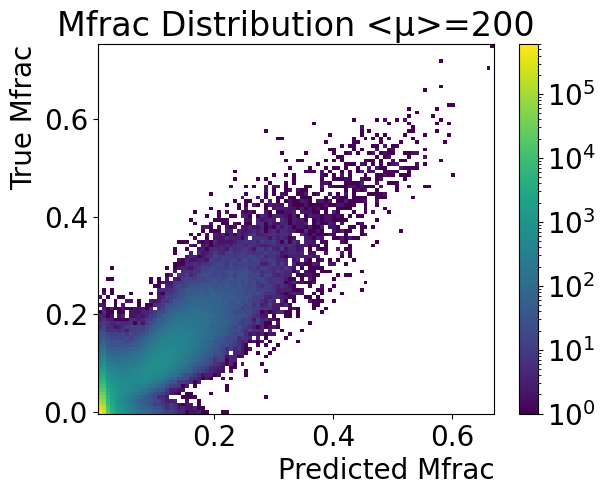
\includegraphics[width=1\linewidth]{Mfrac2D_mu200.png}
  \caption{}
  \label{fig:Mfrac2d_mu200}
\end{subfigure}
\caption{At $\left \langle \mu \right \rangle=60$ (top row) and $\left \langle \mu \right \rangle=200$ (bottom row), the predicted energy (left) and mass (right) fraction of jets shown as 1D and 2D histograms.}
\label{fig:RegressionResults}
\end{figure}

\textbf{Regression Results:} \myname{} was evaluated on a sample of 20k di-Higgs events simulated specifically for testing. At $\left \langle \mu \right \rangle=60$, the model achieves $R^2=0.916$ for $E_{frac}$, as shown in Figure~\ref{fig:Efrac1d_mu60}, and $R^2=0.757$ for $M_{frac}$, as shown in Figure~\ref{fig:Mfrac1d_mu60}. At $\left \langle \mu \right \rangle=200$, the model achieves $R^2=0.912$ for $E_{frac}$, as shown in Figure \ref{fig:Efrac1d_mu200}, and $R^2=0.720$ for $M_{frac}$, as shown in Figure \ref{fig:Mfrac1d_mu200}. The 2D predicted vs truth values, plotted with a log z color scale, shown in Figure [\ref{fig:Efrac2d_mu60},\ref{fig:Mfrac2d_mu60}] at $\left \langle \mu \right \rangle=60$ and in Figure \ref{fig:Efrac2d_mu200} \ref{fig:Mfrac2d_mu200} at $\left \langle \mu \right \rangle=200$, show that there is good diagonal trend between the predictions and the truth. Overall, the transformer encoder architecture provides a highly parallelizable algorithm that is computationally feasible at high pileup conditions, and the plots in Figure~\ref{fig:RegressionResults} show that \myname{} learns the hard scatter contributions without significant degradation to the $R^2$ value at high pileup conditions of the HL-LHC.

%\luke{Move part of this discussion to the Jet Labels section}It is clear from the 2D histograms that the model performs noticeably better on Efrac than Mfrac, which is expected due to the physics. Energy fraction is analogous to a scalar sum while mass fraction is analogous to vector sum. Pileup contamination typically has low energy and therefore does not affect the scalar sum as much as the stochastic direction vectors affect the vectorial sum used to calculate mass fraction. The model is very good at identifying hard scatter jets, with energy fraction close to one, but the model does not perform as well with pileup jets, energy fraction close zero. However, its important to note that the hard scatter jets are of most interest to physics, and there is very good energy fraction modeling in this region. \\

\newpage
\textbf{Classic JVT Benchmark:} In order to benchmark the performance of the model against existing JVT algorithm, only a subset of the model is used to maintain consistency across input features. For a fair comparison, only jet features are considered: \{$p_T,\eta,\phi,m,R_{p_T},corrJVF$\} where $R_{p_T}$ and $corrJVT$ are defined in ~\cite{ATLAS-CONF-2014-018}. This exercise attempts to show that the attention architecture over jet features (AttnJVT) alone brings noticeable improvements when jets are processed in the context of an event. These results can be further improved when jets are compounded with track features.

\begin{figure}[ht]
\centering
\begin{subfigure}{.32\textwidth}
  \centering
  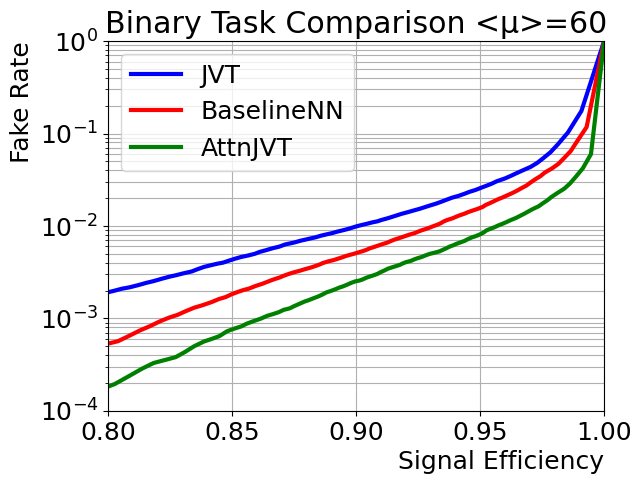
\includegraphics[width=1\linewidth]{JVT_Benchmark_mu60.png}
  \caption{}
  \label{fig:Benchmark:sub1}
\end{subfigure}%
\begin{subfigure}{.32\textwidth}
  \centering
  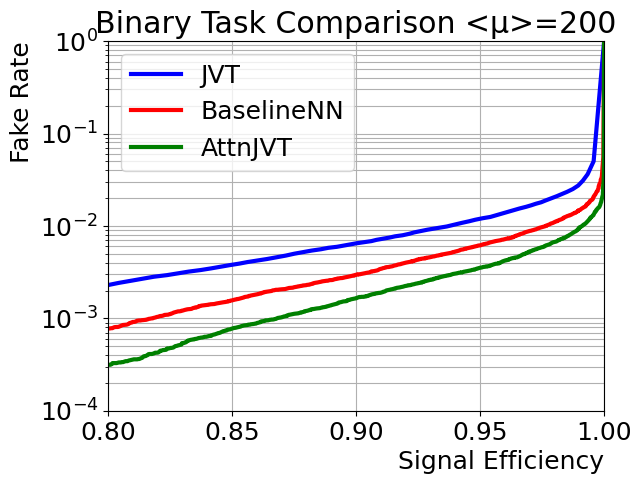
\includegraphics[width=1\linewidth]{JVT_Benchmark_mu200.png}
  \caption{}
  \label{fig:Benchmark:sub2}
\end{subfigure}
\begin{subfigure}{.32\textwidth}
  \centering
  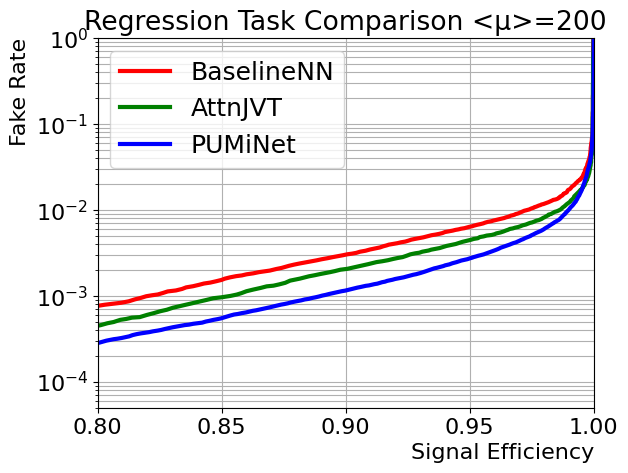
\includegraphics[width=1\linewidth]{ROC_Comparison_wtracks.png}
  \caption{}
  \label{fig:Benchmark:sub3}
\end{subfigure}
\caption{Benchmark performance for the binary classification task for replica ATLAS JVT (blue), baseline deep NN (red), and MHA jet encoder (green) for for $\left<\mu\right>=60$ (a) and $\left<\mu\right>=200$ (b). Further improvement can be gained by \myname{} when tracks are added to the model (c). }
\label{fig:Benchmark}
\end{figure}

Using the di-Higgs dataset, the following models were created: (1) a replica of ATLAS JVT kNN model described in ~\cite{ATLAS-CONF-2014-018} (2) a baseline deep neural network, and (3) a single MHA encoder between jets, AttnJVT.\footnote{A small number of learnable parameters are used, 21k, for AttnJVT and the baseline deep NN.} Since JVT is a binary classifier, the continuous labels are converted to binary using a cut at $E_{frac}=0.3$. The JVT algorithm and deep NN process inputs on a per jet basis, but AttnJVT processes an entire set of jets in the context of an event which allows the model to capture correlations between hard scatter jets. The baseline deep NN and AttnJVT are trained using the Binary Cross Entropy loss function, and converges after 60 epochs on 50k events. The benchmarked false positive rates against the true positive rates are shown in Figure Figure \ref{fig:Benchmark:sub1} \& \ref{fig:Benchmark:sub2} which shows that AttnJVT can significantly lower the false positive rate. We also show that \myname{} brings further improvements over AttnJVT using both jet and track features to capture event-wide correlations in the regression setup, as shown in Figure \ref{fig:Benchmark:sub3}.


\section{Analysis}\hfill

In order to determine if the model is able to provide useful insight into a practical physics analysis, we attempt to reconstruct the Higgs mass from DiHiggs decaying to 4b events with a non-resonant 4b background. The non-resonant 4b sample has a 60GeV pTB filter applied at generation level to ensure the kinematics of each sample are indistinguishable. Therefore, the only difference between these samples is the the resonant mass peak that appears in the DiHiggs sample and the flat background from the non-resonant 4b sample.

Using the results of the Efrac and Mfrac model, we are able to apply jet corrections and see 

\begin{figure}[h!]
    \centering
    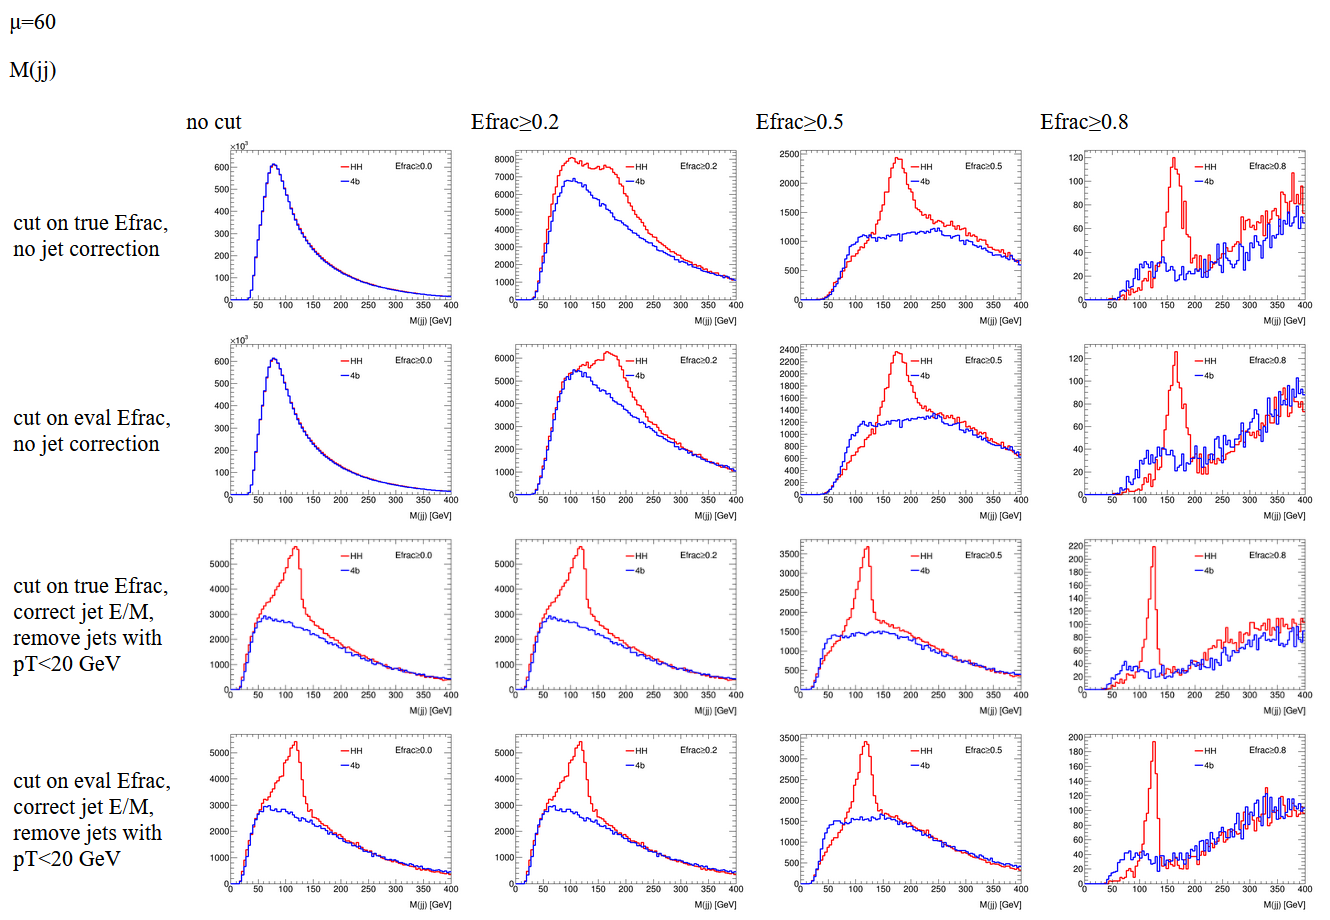
\includegraphics[width=1\linewidth]{tmp.png}
    \caption{Physics Analysis Results}
\end{figure}


\section{Conclusion}\hfill

We suggest a novel model, \myname{}, to address the effect of the pileup interactions on physics studies at the current and future LHC conditions. The model makes use of a set of transformers with self- and cross-attention with the input of track and jet parameters in the event. The proposed architecture allows the model to learn kinematic correlations arising from physics processes, which helps to recover the hard scatter process properties. As the output, \myname{} predicts the fractions of jet energy and jet mass due to pileup. The model was trained and tested using simulated di-Higgs datasets. It was shown that the model is capable of recovering the value and resolution of the Higgs boson mass in high-pileup conditions, where initially the Higgs boson mass peak is not possible to observe. \myname{} also scales well with the expected increase of the pileup level at the LHC and HL-LHC.

%The LHC prepares to upgrade to the HL-LHC phase which brings significantly more pileup contamination to hard scatter jets. To mitigate the effects of high pileup conditions, we introduce $E_{frac}$ and $M_{frac}$ to perform direct identification, energy, and mass correction of hard scatter jets. We train the proposed method on a regression task to directly predict $E_{frac}$ and $M_{frac}$ through a diHiggs simulated dataset. The model uses transformer encoders using self and cross attention to enrich representations of jet features using all possible correlations between jet and tracks within the context of an event. We show that this model scales well in high pileup conditions, and through extensive analysis we show that the expected Higgs mass resonance can be restored and the effects of pileup can be mitigated. Lastly, $E_{frac}$ and $M_{frac}$ can be used as physically significant features and increase performance and a direct binary classification task using an attention architecture. 

%In conclusion, we presented the following contributions.
%\begin{enumerate}
%    \item We proposed a first-of-its-kind pileup prediction modeled as a regression problem.
%    \item We proposed a cross-attention based neural network architecture that utilizes jets and tracks information for pileup fraction detection.
%    \item We showed with extensive analysis that the proposed method outperforms the baseline approaches.
%    \item We also showed that the predictions from the proposed approach also assist with physics processes.
%\end{enumerate}
%
% ---- Bibliography ----
%
% BibTeX users should specify bibliography style 'splncs04'.
% References will then be sorted and formatted in the correct style.
%
\bibliographystyle{splncs04}
\bibliography{bibliography}
%
\end{document}
